\documentclass[10pt,openany]{report}
\usepackage[a4paper,margin=1in]{geometry}
\usepackage{lmodern}
\usepackage[T1]{fontenc}
\usepackage{textcomp}
\usepackage{amsmath,amssymb}
\usepackage{graphicx}
\usepackage{booktabs}
\usepackage{array}
\usepackage{longtable}
\usepackage{multicol}
\usepackage{float}
\usepackage{tikz}
\usepackage{xcolor}
\usepackage{setspace}
\usepackage{caption}
\usepackage{hyperref}
\usepackage{enumitem}
\usetikzlibrary{shapes.geometric,arrows.meta,positioning,fit,backgrounds,calc,decorations.pathreplacing}

\hypersetup{
  colorlinks=true,
  linkcolor=black,
  citecolor=black,
  urlcolor=blue!45!black,
  pdftitle={GlandersWatch: A Modular Platform for Glanders Risk Prediction, Retrieval-Augmented Explanation and Owner Alerting},
  pdfauthor={Pedapatruni Shanmukh Vardhan, Shaktimayee Mohanty, Yuvraj Singh},
  pdfsubject={B.Tech Project Report, International Institute of Information Technology, Bhubaneswar}
}

\graphicspath{{figures/}}
\def\GlandersWatchReport{}
\captionsetup{font=small,labelfont=bf,skip=6pt}
\setlength{\parskip}{0.35em}
\setlength{\parindent}{0pt}
\setlength{\emergencystretch}{1.5em}
% single spacing, as in the department template

% Section numbering follows the department template: sections are "1.", "2." within
% each chapter (counter resets per chapter) and subsections are "1.1", "1.2".
\renewcommand{\thesection}{\arabic{section}.}
\renewcommand{\thesubsection}{\arabic{section}.\arabic{subsection}}

% chapter-based numbering for floats and equations
\counterwithin{figure}{chapter}
\counterwithin{table}{chapter}
\renewcommand{\thefigure}{\thechapter.\arabic{figure}}
\renewcommand{\thetable}{\thechapter.\arabic{table}}

% 
\tikzset{
  src/.style={rectangle,rounded corners=2pt,draw=blue!55!black,fill=blue!7,
              align=center,minimum height=0.62cm,text width=2.55cm,
              font=\scriptsize\sffamily,inner sep=3pt},
  proc/.style={rectangle,rounded corners=2pt,draw=black!55,fill=black!4,
               align=center,minimum height=0.62cm,text width=2.55cm,
               font=\scriptsize\sffamily,inner sep=3pt},
  dec/.style={diamond,draw=orange!70!black,fill=orange!10,aspect=2.1,
              align=center,font=\scriptsize\sffamily,inner sep=1.5pt},
  res/.style={rectangle,rounded corners=2pt,draw=teal!60!black,fill=teal!8,
              align=center,minimum height=0.62cm,text width=2.55cm,
              font=\scriptsize\sffamily,inner sep=3pt},
  arr/.style={-{Stealth[length=1.8mm]},thick,draw=black!65},
  darr/.style={-{Stealth[length=1.8mm]},thick,dashed,draw=black!45},
  lbl/.style={font=\scriptsize\sffamily,inner sep=1.5pt,fill=white,align=center},
  grp/.style={rectangle,rounded corners=4pt,draw=black!25,fill=black!2,
              inner sep=6pt},
  hdr/.style={font=\scriptsize\sffamily\bfseries,anchor=south west,inner sep=1pt},
}

\begin{document}
% The department template numbers continuously in arabic from the Certificate page,
% with the title page carrying no number, so Abstract falls on page 4.
\pagenumbering{arabic}
\setcounter{page}{0}

% ============================== TITLE PAGE ==============================
% Bold/regular pattern measured from the department template: the title is large but
% REGULAR weight; the four structural headings are bold; author names are bold with the
% roll numbers set regular in a second column. Names right-aligned, roll numbers
% left-aligned, as a tabular{rl}.
\begin{titlepage}
\thispagestyle{empty}
\begin{center}

{\huge GlandersWatch: A Modular Platform for\\[7pt]
Glanders Risk Prediction, Retrieval-Augmented\\[7pt]
Explanation and Owner Alerting\par}

\vspace{1.15cm}

{\Large\bfseries Project Report Submitted\par}
\vspace{0.30em}
{\normalsize in partial fulfillment of the requirements for the award of the\par}

\vspace{1.05cm}
{\Large\bfseries Bachelor of Technology\par}
\vspace{0.28em}
{\normalsize in\par}
\vspace{0.22em}
{\Large\bfseries Computer Science Engineering\par}

\vspace{0.95cm}
{\normalsize by\par}
\vspace{0.40em}
{\fontsize{10.9}{13.2}\selectfont
\begin{tabular}{@{}r@{\hspace{1.1em}}l@{}}
\bfseries Pedapatruni Shanmukh Vardhan & B123089 \\[1pt]
\bfseries Shaktimayee Mohanty & B123118 \\[1pt]
\bfseries Yuvraj Singh & B123153 \\
\end{tabular}\par}

\vspace{1.0cm}
{\normalsize Under the supervision of\par}
\vspace{0.32em}
{\fontsize{10.9}{13.2}\selectfont\bfseries Dr. Sangita Dhara\par}

\vspace{1.0cm}

\includegraphics[width=3.0cm]{iiit_logo.png}\par

\vfill

{\normalsize Department of Computer Science and Engineering\par}
\vspace{0.32em}
{\fontsize{10.9}{13.2}\selectfont\bfseries International Institute of Information Technology, Bhubaneswar\par}
\vspace{0.32em}
{\normalsize November 2026\par}

\vspace*{0.6cm}

\end{center}
\end{titlepage}

% ============================== CERTIFICATE ==============================
\newpage
\thispagestyle{empty}
\noindent\underline{\textbf{Certificate}}

\vspace{0.9cm}
\noindent
{\sloppy
This is to certify that the report entitled ``GlandersWatch: A Modular Platform for Glanders Risk
Prediction, Retrieval-Augmented Explanation and Owner Alerting'' submitted by \mbox{Pedapatruni Shanmukh Vardhan (B123089)}, \mbox{Shaktimayee Mohanty (B123118)} and \mbox{Yuvraj Singh (B123153)} to
International Institute of Information Technology, Bhubaneswar is a record of bonafide project work
under my supervision, and the report is submitted for the evaluation of the BTech
Degree Final-Semester Project.\par}

\vspace{1.5cm}
\noindent
Dr. Sangita Dhara\\[0.2em]
\underline{(Supervisor)}

% ============================== DECLARATION ==============================
\newpage
\thispagestyle{empty}
\noindent\underline{\textbf{Declaration}}

\vspace{0.9cm}
\noindent
We certify that

\begin{enumerate}
  \item The work contained in the report has been done by ourselves under the general supervision
        of our supervisor.
  \item The work has not been submitted to any other Institute for any degree or diploma.
  \item We have followed the guidelines provided by the Institute in writing the report.
  \item We have conformed to the norms and guidelines given in the Ethical Code of Conduct of the
        Institute.
  \item Whenever we have used materials (data, theoretical analysis, and text) from other sources,
        we have given due credit to them by citing them in the text of the report and giving their
        details in the references.
  \item Whenever we have quoted written materials from other sources, we have put them under
        quotation marks and given due credit to the sources by citing them and giving required
        details in the references.
\end{enumerate}

\vspace{2.5cm}
\noindent
\noindent
\begin{tabular}{@{}p{5.75cm}p{4.35cm}p{4.35cm}@{}}
\textbf{Pedapatruni Shanmukh Vardhan} & \textbf{Shaktimayee Mohanty} & \textbf{Yuvraj Singh} \\[0.12em]
B123089 & B123118 & B123153 \\
\end{tabular}

% ============================== ACKNOWLEDGMENTS ==============================
\newpage
\thispagestyle{empty}
\noindent\underline{\textbf{Acknowledgments}}

\vspace{0.9cm}
\noindent
We would like to express our sincere gratitude to our respected supervisor, Dr. Sangita Dhara, for the
invaluable guidance, support and encouragement given throughout this project. Her insights and
expertise were instrumental in shaping this work and helped us overcome numerous challenges. We are
also thankful to the faculty and staff of the Department of Computer Science and Engineering,
International Institute of Information Technology, Bhubaneswar, for providing the resources and a
conducive learning environment. Finally, we would like to thank our families and friends for their
unwavering support and understanding during the course of this project.

\vspace{2.5cm}
\noindent
\noindent
\begin{tabular}{@{}p{5.75cm}p{4.35cm}p{4.35cm}@{}}
\textbf{Pedapatruni Shanmukh Vardhan} & \textbf{Shaktimayee Mohanty} & \textbf{Yuvraj Singh} \\[0.12em]
B123089 & B123118 & B123153 \\
\end{tabular}

% ============================== ABSTRACT ==============================
\newpage
\pagestyle{plain}
\noindent\underline{\textbf{Abstract}}
\addcontentsline{toc}{chapter}{Abstract}

\vspace{0.7cm}
\noindent
Glanders is a bacterial zoonosis of equids caused by \textit{Burkholderia mallei}. It is
notifiable, frequently fatal, and remains endemic in parts of Africa, Asia and South America.
Indian surveillance between 2019 and 2023 identified 728 seropositive equids across 138 districts,
with strong geographic concentration. A district officer and an equine owner both need more than a
retrospective case count: they need a usable forecast for the next period, a way to ask what official
guidance requires, and messages sparse enough that people still read them. The published machine
learning literature on this disease is confined to laboratory identification of the organism; no
population-level geographic risk model, and no owner-facing warning path, has been reported.

\vspace{0.5em}
\noindent
This report presents GlandersWatch as three independently deployable components. A calibrated risk
engine forecasts whether glanders is documented in a country in year $t{+}1$ from features observed
in year $t$. A retrieval-augmented generation (RAG) layer answers questions from officers or owners
using passages retrieved from official guidance: every claim must cite a retrieved passage, and the
layer refuses when the corpus does not support an answer. An alert service decides whether a message
should be sent at all (thresholding, hysteresis, suppression and deduplication) so volume stays low
enough that messages are still read. Components talk through versioned schemas rather than shared
internals; none hardcodes the disease; and each can degrade without taking the others down.

\vspace{0.5em}
\noindent
The risk engine combines four public datasets not previously applied to glanders into a country-year
panel: a text-mined occurrence corpus from Europe PMC, FAOSTAT livestock stocks, World Bank
development indicators and NASA POWER reanalysis climatology. 6,700 country-year rows reduce to
2,880 modelling observations across 160 equine-holding countries from 2005 to 2023, with
169 positive labels. Eight of 42 numeric candidates are retained by mean absolute SHAP on the
training years alone, and six model families are compared under temporal and leave-country-out
validation. On unseen years the strongest precision-recall AUC is 0.495 against a 5.87\% base rate;
on unseen countries the ranking inverts and Logistic Regression leads at 0.381 with calibration
error 0.025, so it is the champion for deployment.

\vspace{0.5em}
\noindent
The RAG layer is specified as hybrid retrieval over official guidance, with citation checks and
refusal rules. The alert service is specified as a period-aware rules engine with replaceable
delivery adapters. Neither has measured field performance yet, because neither is deployed; the
interfaces, rules and evaluation protocol are fixed so a later pilot can score them. The main
limitation of the model is the label itself: a positive means documentation, not incidence, so
reporting effort is the principal confounder and the main target for future work.

\vspace{0.7em}
\noindent
\textbf{Keywords:} Glanders, \textit{Burkholderia mallei}, Risk Prediction, Gradient Boosting,
Probability Calibration, SHAP, Retrieval-Augmented Generation, Citation Grounding, Alert Fatigue,
Modular System Design, Animal Health Surveillance.

% ============================== CONTENTS ==============================
\newpage
\pagestyle{plain}
\noindent\underline{\textbf{Contents}}
\vspace{0.55cm}

% \tableofcontents would insert its own chapter-style heading and a page break;
% \@starttoc typesets the entries alone, under the heading above.
\makeatletter
\@starttoc{toc}
\makeatother

% =====================================================================
\chapter{Introduction}
\label{ch:intro}
% =====================================================================

\section{Background}

Glanders is a contagious and often fatal disease of horses, donkeys and mules caused by
\textit{Burkholderia mallei}. The organism has no environmental reservoir, and asymptomatic
carriers remain infectious for long periods. Human infection is rare but carries a high case
fatality rate and follows occupational contact. The disease is notifiable to the World
Organisation for Animal Health and is classified as a potential bioterrorism agent.

The economic weight sits in low and middle income countries, where equids remain essential to
transport, construction and agriculture. An equid is a member of the family \emph{Equidae}: horses,
donkeys (recorded here as asses) and mules. India held 5.50 lakh of them in the 2019 Livestock
Census, made up of 3.42 lakh horses, 1.24 lakh asses and 0.84 lakh mules. That figure is the size of
the susceptible population, not a count of sick animals: it says how many animals are exposed, not how
many the disease has damaged. Most are held by households that depend on them for daily income, so the
death of one working animal is a direct loss of livelihood.

The damage that is documented is smaller and better measured. A national programme screening
158,798 sera from 391 districts between 2019 and 2023 found 728 seropositive animals in 138 districts,
roughly sixty per cent of them in Uttar Pradesh; earlier surveillance covering 2006 to 2018 reported
1,145 positives among 128,404 sera. That is under one per cent of the equid population, concentrated
in a few states, and because glanders is notifiable and frequently fatal once clinical, each positive
is acted on rather than monitored.

\begin{figure}[htbp]
\centering
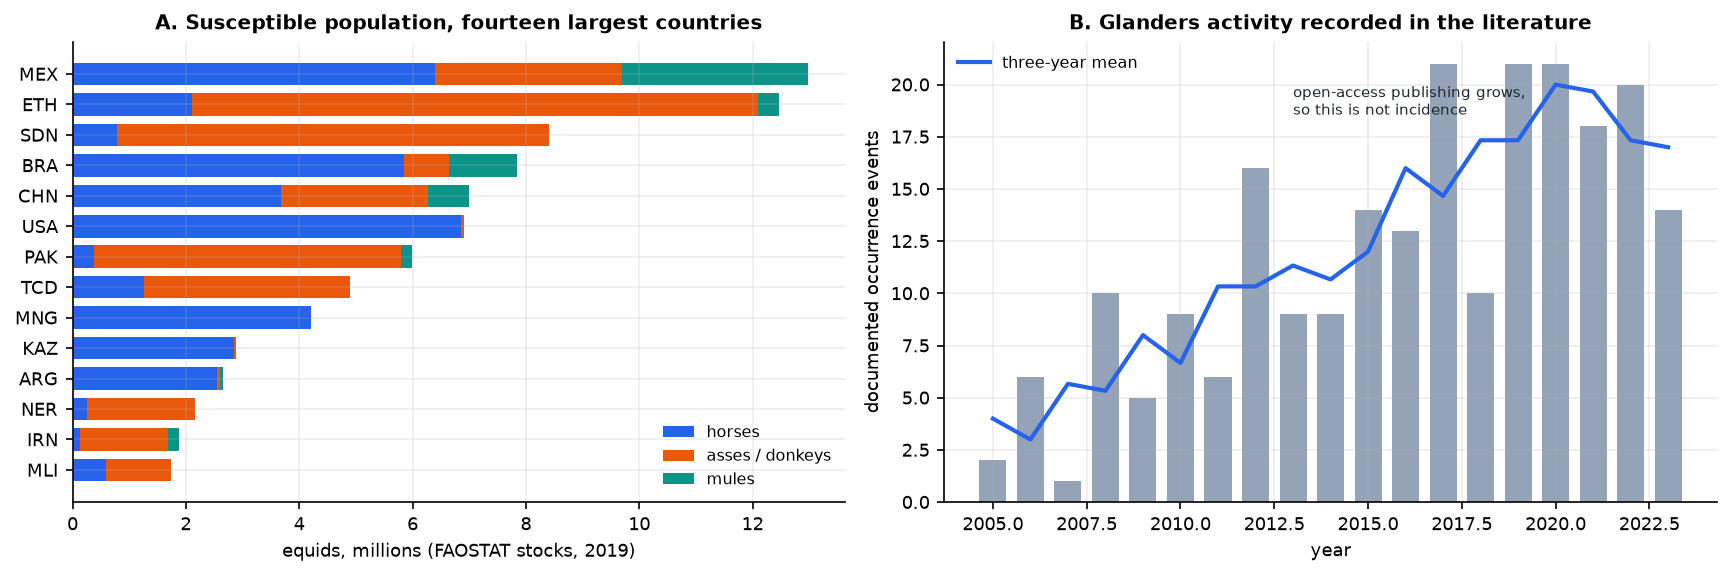
\includegraphics[width=0.95\textwidth]{fig14_background.png}
\caption{The two quantities behind the problem. Panel A gives the equid population of the fourteen
largest countries, split by species, which sets the size of the exposed population. Panel B gives the
occurrence events recovered from the literature each year, which sets the size of the label. The rise
in panel B follows open-access publishing volume as much as disease, which is why the label is treated
as documented activity throughout.}
\label{fig:background}
\end{figure}

\section{Problem Definition}

A district veterinary officer faces a narrow question: is glanders likely to appear in this area
in the coming year? The task is framed as supervised classification on a country-year panel:
features observed in year $t$ predict a binary label for year $t{+}1$. Answering it means combining
the history of the disease nearby, the size of the susceptible population, and the conditions that
permit transmission.

Surveillance reports what has already happened, and forecasting systems exist for several livestock
diseases but not for glanders. A probability alone is still hard to use in the field: an owner needs
to ask what to do next, and an officer needs answers that can be checked against official guidance.
A warning that arrives for every area every month also teaches its recipients to ignore it.

The problem therefore has four parts, two concerned with producing the prediction and two with what
happens after it.

\begin{enumerate}
  \item \textbf{Data and label.} No public source records glanders occurrence completely, so
        occurrence must be reconstructed from the literature and joined to population and
        environmental covariates at a common resolution. The outcome is then rare, so accuracy is
        a poor summary statistic, and a negative observation needs an explicit meaning.
  \item \textbf{Model selection under distribution shift.} A model fitted on some countries must be
        evaluated on countries it has never seen, because that is the deployment condition.
  \item \textbf{Grounded question answering.} Officers and owners need to ask questions about
        control measures, reporting duties and next steps, and receive answers grounded in official
        guidance. Claims must cite retrieved passages; if the corpus does not support an answer, the
        system should refuse rather than invent one.
  \item \textbf{Delivery without alert fatigue.} A probability is not an alert, so the operating
        point and the message rules must keep volume low enough that messages are read while the
        threshold stays defensible against the events caught.
\end{enumerate}

\section{Objectives}

The project has three objectives.

\begin{enumerate}
  \item \textbf{Prediction as a service.} Package a calibrated next-year risk model as a versioned
        artefact behind a REST interface, so any consumer can call it without knowing how it works.
  \item \textbf{Grounded Q\&A.} Build a retrieval-augmented layer that answers questions from
        official guidance, cites every claim, and refuses rather than guesses.
  \item \textbf{Owner alerts.} Convert a calibrated probability into few enough messages that they
        are read, using threshold, suppression and deduplication rules.
\end{enumerate}

All three share one requirement: each component must be independently testable and replaceable, and
must not hardcode glanders into its core logic.

\section{Scope}

The study is scoped to country-year resolution. District-level modelling for India was envisaged but
is not attempted, because the covariates could not be assembled from public sources within the project
period. The RAG and alert layers do not depend on that resolution and can sit in front of a
district-level model later without redesign. The model is a population-level tool: it does not
diagnose an individual animal and does not replace laboratory confirmation. Limitations that shape
the results are collected in Section~\ref{sec:limitations}.

% =====================================================================
\chapter{Literature Review and Gap Analysis}
\label{ch:lit}
% =====================================================================

\section{Epidemiology and Surveillance}

Glanders is treated as a neglected zoonosis with high case fatality and a real occupational risk to
handlers \cite{khan2013,kanani2026}. A recent systematic review and meta-analysis consolidates
seroprevalence estimates and identifies management practice and animal movement as the dominant
drivers \cite{purnama2026}; regional reviews document continued circulation in Brazil
\cite{mota2022}. The disease persists where equid populations are large, animals move often and
surveillance is weak. The first two are measurable from public data, while the third decides whether
the disease is visible at all and is therefore a confounder rather than a covariate.

Indian surveillance is the strongest evidence base. Malik et al. described outbreaks reported
between 2006 and 2011 \cite{malik2012}, Singha et al. reported serological surveillance for 2015 to
2018 \cite{singha2020}, and the national programme covering 2019 to 2023 produced a prevalence
estimate with a risk analysis \cite{singha2026}. These establish where glanders occurs and which
animal-level factors the risk analysis identified. None builds a predictive model, and none uses
population or reanalysis covariates as predictors.

\section{Existing Forecasting Systems in India}

The closest operational system is NADRES v2, the National Animal Disease Referral Expert System run
by ICAR-NIVEDI \cite{nadres}. It combines outbreak records from AICRP centres with meteorological and
remote-sensing covariates and issues district-level forewarnings about two months ahead, using a
model family that overlaps with the one used here.

This project differs in four complementary ways. It is glanders-specific, where a national system
must spread effort across many diseases. It uses only public data, so anyone can reproduce and audit
it. It adds a question-answering layer over official guidance, which matters when the reader is an
owner rather than a trained analyst. And it delivers to the owner directly, with rules that suppress
routine noise. NADRES has institutional access this project lacks; this project spends that
difference on local Q\&A and owner delivery that a multi-disease platform does not attempt.

\section{Glanders Risk Modelling and Related Machine Learning}

Spatial work on glanders is descriptive: Fonseca-Rodr\'iguez et al.\ applied spatiotemporal cluster
detection to Brazilian data \cite{fonseca2019}, which identifies where cases have already
concentrated but does not predict which units will be positive in the next period.

Indian surveillance studies establish prevalence and animal-level factors but stop short of a forward
model: Malik et al.\ on 2006--2011 outbreaks \cite{malik2012}, Singha et al.\ on 2015--2018
serology \cite{singha2020}, and the 2019--2023 national programme with risk analysis
\cite{singha2026}. NADRES v2 issues multi-disease livestock forewarnings \cite{nadres}; it is the
closest operational comparator, but is not glanders-specific and does not deliver cited owner alerts
from public data alone.

The only machine learning work specific to \textit{B. mallei} is spectroscopic identification.
Moawad et al.\ built a Raman assay with learned classifiers \cite{moawad2019}, and St\"ockel et al.\
reported spectroscopic detection of \textit{B. mallei} and \textit{B. pseudomallei}
\cite{stoeckel2015}. Both are laboratory diagnostic problems; neither produces a population risk
estimate. Using published literature as structured occurrence data has precedent in epidemic
intelligence \cite{collier2012,lejeune2015}; here extraction is the primary label source because
official outbreak records are incomplete for many countries, so reporting bias is analysed rather
than assumed away.

Because no glanders study compares model families on a shared panel, the evaluation design draws on
method papers that are not disease-specific: how to compare classifiers under imbalance
\cite{saito2015,davis2006}, how to split data with spatial structure so country identity cannot leak
\cite{roberts2017}, how to attribute predictions across features \cite{lundberg2017}, and how to
judge whether predicted probabilities are usable as probabilities \cite{niculescu2005,huang2020}.
Those references justify the metrics and splits used in Chapter~\ref{ch:method}; they are not prior
glanders risk models.

\begin{table}[htbp]
\centering
\caption{Comparative summary for the risk engine. Upper rows are glanders (or glanders-organism)
studies; lower rows are method papers that guide multi-model evaluation.}
\label{tab:ml-compare}
\small
\begin{tabular}{@{}>{\raggedright\arraybackslash}p{2.55cm}
                >{\raggedright\arraybackslash}p{3.35cm}
                >{\raggedright\arraybackslash}p{3.15cm}
                >{\raggedright\arraybackslash}p{3.55cm}@{}}
\toprule
\textbf{Study} & \textbf{Approach} & \textbf{Problem addressed} & \textbf{Limitation} \\
\midrule
Fonseca-Rodr\'iguez et al.\ (2019) &
Spatiotemporal cluster detection on Brazilian glanders records &
Where cases have already concentrated &
Describes past clusters; no next-period prediction \\
Singha et al.\ (2020, 2026); Malik et al.\ (2012) &
Serological surveillance and outbreak description in India &
Prevalence and risk factors in equids &
No forward predictive model on a covariate panel \\
NADRES v2 \cite{nadres} &
Multi-disease livestock forewarning &
District-level early warning across diseases &
Not glanders-specific; owner-facing cited delivery out of scope \\
Moawad et al.\ (2019); St\"ockel et al.\ (2015) &
Raman / spectroscopic classifiers for \textit{B.\ mallei} &
Laboratory identification of the organism &
Diagnostic, not geographic risk \\
\midrule
Saito and Rehmsmeier (2015); Davis and Goadrich (2006) &
Precision--recall versus ROC analysis &
How to score rare-event classifiers &
Method only; no glanders application \\
Roberts et al.\ (2017) &
Cross-validation for structured spatial / temporal data &
Honest holdouts when units are correlated &
Method only; guides leave-country-out here \\
Lundberg and Lee (2017) &
SHAP feature attribution &
Comparing what models use, across families &
Attribution tool, not a disease model \\
Niculescu-Mizil and Caruana (2005); Huang et al.\ (2020) &
Probability calibration measures &
When a score can be read as a probability &
Needed for alert thresholds; not glanders-specific \\
\bottomrule
\end{tabular}
\end{table}

\section{Question Answering and Retrieval-Augmented Generation}

No glanders-specific question-answering system was found. The layer therefore follows general
retrieval-augmented generation practice: retrieve passages, then answer only from those passages
\cite{lewis2020}. Dense embeddings \cite{reimers2019}, lexical retrieval \cite{robertson2009} and
reciprocal rank fusion \cite{cormack2009} are the usual building blocks; none of them is a glanders
product. What is missing is the application: a service that answers veterinary and owner questions
from official control guidance, cites its sources, and refuses when the corpus does not support a
claim. The risk score may be passed in as context for a question; the layer's job is still to answer
the question, not to narrate the score.

\begin{table}[htbp]
\centering
\caption{Related work for the RAG question-answering layer. There is no glanders-specific prior;
rows are the methods adapted here.}
\label{tab:rag-compare}
\small
\begin{tabular}{@{}>{\raggedright\arraybackslash}p{3.0cm}
                >{\raggedright\arraybackslash}p{3.6cm}
                >{\raggedright\arraybackslash}p{3.0cm}
                >{\raggedright\arraybackslash}p{3.2cm}@{}}
\toprule
\textbf{Work} & \textbf{Approach} & \textbf{Problem addressed} & \textbf{Gap for this project} \\
\midrule
Lewis et al.\ (2020) &
Retrieval-augmented generation &
Knowledge-intensive NLP with evidence &
Not wired to a veterinary Q\&A workflow over statutory guidance \\
Reimers and Gurevych (2019) &
Sentence embeddings for semantic search &
Dense passage retrieval &
Retrieval only; no citation or refusal protocol \\
Robertson and Zaragoza (2009) &
BM25 lexical ranking &
Keyword retrieval &
Misses paraphrases; used here only as one hybrid channel \\
Cormack et al.\ (2009) &
Reciprocal rank fusion &
Combining ranked lists &
Fusion method; not an end-to-end veterinary Q\&A service \\
\bottomrule
\end{tabular}
\end{table}

\section{Alerting and Warning Systems}

Related warning systems address pieces of delivery rather than a glanders risk-to-owner path: NADRES
emphasises structured disease reporting, public flood warnings show how to name an area, a level and
an action, early-warning evaluation work stresses receipt and usefulness rather than message send
alone, software alert managers contribute grouping, silencing and routing, and standard public-warning
formats support interchange. None of these is a complete substitute for the service designed here;
Tables~\ref{tab:alert-related-work} and~\ref{tab:alert-comparison} summarise the lessons carried
forward, with implementation detail later in Chapter~\ref{ch:method} (Alerting System).

\begin{table}[htbp]\centering\small
\caption{Previous systems and the lessons applied in GlandersWatch.}\label{tab:alert-related-work}
\begin{tabular}{@{}>{\raggedright\arraybackslash}p{2.7cm}
                >{\raggedright\arraybackslash}p{4.6cm}
                >{\raggedright\arraybackslash}p{5.0cm}@{}}
\toprule
\textbf{Previous work} & \textbf{Main focus} & \textbf{Lesson for GlandersWatch} \\
\midrule
NADRES v2 & Animal-disease surveillance and reporting & Use structured disease information and preserve traceability \\
Google / CWC flood warnings & Hazard communication to affected people & Name area, level and practical action, not only a probability \\
J-PAL Bihar early-warning study & Reach and usefulness of warnings & Evaluate receipt, understanding and response, not only sending \\
Prometheus Alertmanager & Grouping, silencing, inhibition and routing & Control repeats; separate decision from delivery \\
OASIS CAP & Standardised public-warning exchange & Keep alert records structured for possible external integration \\
\bottomrule
\end{tabular}
\end{table}

\begin{table}[htbp]\centering\small
\caption{Difference between reviewed warning work and the proposed alert design.}\label{tab:alert-comparison}
\begin{tabular}{@{}>{\raggedright\arraybackslash}p{2.6cm}
                >{\raggedright\arraybackslash}p{4.9cm}
                >{\raggedright\arraybackslash}p{4.9cm}@{}}
\toprule
\textbf{Aspect} & \textbf{Reviewed work provides} & \textbf{GlandersWatch proposes} \\
\midrule
Input & Surveillance reports, hazard feeds or monitoring alerts & Calibrated glanders risk with area, period, model version and freshness \\
Period & Source-specific frequency & One period-aware contract for monthly and yearly records \\
Risk state & Warning or alert-management primitives & LOW / MEDIUM / HIGH with hysteresis and previous-state comparison \\
Notification control & Routing, silencing or distribution examples & Unchanged-level, cooldown, escalation, stale-data, mute, quiet-hour and daily-cap rules \\
Duplicate control & Grouping or deduplication in some systems & Separate protection for alert, recipient job and send attempt \\
Recipients / delivery & Domain- and platform-specific & Area subscriptions, preferences, queue fan-out and replaceable channel adapters \\
Audit & Varies & Reason-coded sent / skipped decisions and per-recipient delivery history \\
\bottomrule
\end{tabular}
\end{table}

\section{Gaps and Contribution}

Glanders epidemiology and laboratory identification are documented, yet a calibrated next-year
population risk model on a public country-year panel is not. Retrieval-augmented generation is a
mature method, but there is no glanders Q\&A service that answers from official guidance, cites its
sources and refuses when unsupported. Warning and alert-management systems exist in other domains,
but none of them takes a calibrated glanders probability through hysteresis, suppression and
deduplication to consented owner messages with an audit trail.

This project specifies a three-part platform behind fixed contracts: a risk engine that compares
model families under temporal and leave-country-out validation, a RAG layer for grounded question
answering, and an alert service that sends few enough messages to remain readable.
Chapter~\ref{ch:method} develops each part, while Chapter~\ref{ch:results} reports
measured results only for the risk engine.

% =====================================================================
\chapter{System Architecture}
\label{ch:arch}
% =====================================================================

\section{What the Platform Has to Do}

The risk engine answers whether glanders is likely to be documented in an area next period, while
the platform also answers questions through the RAG layer and, when policy allows, delivers a short
message to an owner. Those three jobs have different readers and different failure modes, so putting
them in one process would couple alert delivery to LLM latency and make the risk model hard to test
on its own.


\begin{figure}[htbp]
\centering
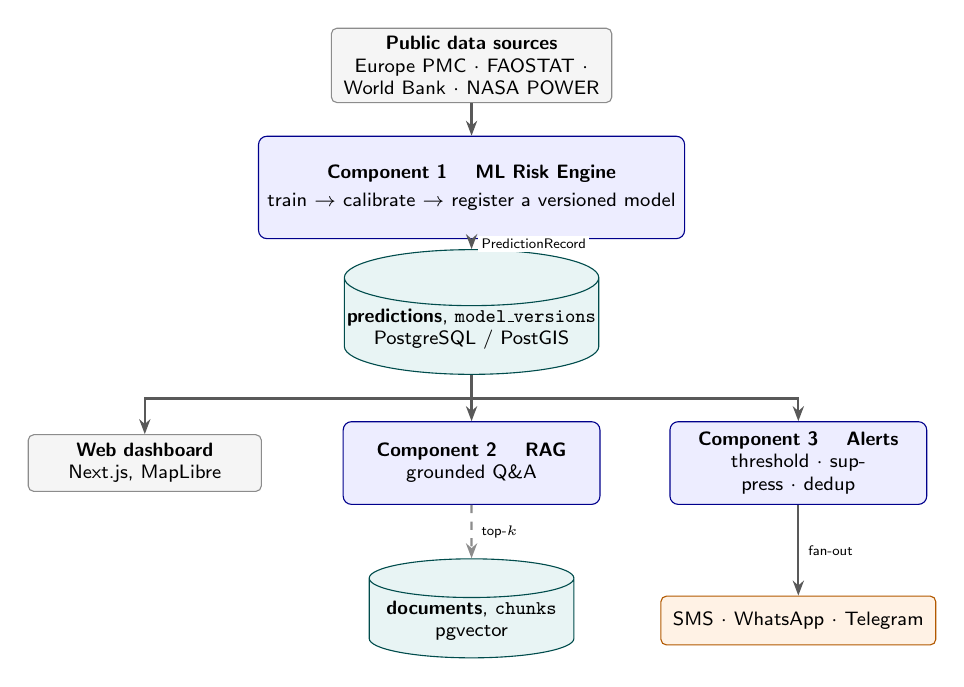
\begin{tikzpicture}[
  comp/.style={rectangle,rounded corners=3pt,draw=blue!55!black,fill=blue!7,
               align=center,minimum height=1.05cm,text width=3.35cm,
               font=\scriptsize\sffamily,inner sep=3pt},
  ext/.style={rectangle,rounded corners=2pt,draw=black!45,fill=black!4,
              align=center,minimum height=0.72cm,text width=3.35cm,
              font=\scriptsize\sffamily,inner sep=3pt},
  store/.style={cylinder,draw=teal!60!black,fill=teal!9,shape border rotate=90,
                aspect=0.22,minimum width=3.1cm,minimum height=1.15cm,
                font=\scriptsize\sffamily,align=center,inner sep=1pt},
  chan/.style={rectangle,rounded corners=2pt,draw=orange!70!black,fill=orange!10,
               align=center,minimum height=0.62cm,text width=3.35cm,
               font=\scriptsize\sffamily,inner sep=2pt},
  fl/.style={-{Stealth[length=1.9mm]},thick,draw=black!65},
  dfl/.style={-{Stealth[length=1.9mm]},thick,dashed,draw=black!45},
  clbl/.style={font=\tiny\sffamily,fill=white,inner sep=1.2pt,align=center},
]

  % ---- sources -----------------------------------------------------------
  \node[ext] (src) at (0,0)
    {\textbf{Public data sources}\\ Europe PMC $\cdot$ FAOSTAT $\cdot$ World Bank $\cdot$ NASA POWER};

  % ---- component 1 -------------------------------------------------------
  \node[comp,minimum height=1.30cm,text width=5.2cm] (c1) at (0,-1.55)
    {\textbf{Component 1 \quad ML Risk Engine}\\[2pt]
     train $\rightarrow$ calibrate $\rightarrow$ register a versioned model};

  % ---- prediction store --------------------------------------------------
  \node[store] (db) at (0,-3.35)
    {\textbf{predictions}, \texttt{model\_versions}\\
     PostgreSQL / PostGIS};

  % ---- the three consumers ----------------------------------------------
  \node[ext,text width=2.75cm] (dash) at (-4.15,-5.05)
    {\textbf{Web dashboard}\\ Next.js, MapLibre};

  \node[comp,text width=3.05cm] (c2) at (0,-5.05)
    {\textbf{Component 2 \quad RAG}\\ grounded Q\&A};

  \node[comp,text width=3.05cm] (c3) at (4.15,-5.05)
    {\textbf{Component 3 \quad Alerts}\\ threshold $\cdot$ suppress $\cdot$ dedup};

  % ---- leaf stores -------------------------------------------------------
  \node[store,minimum width=2.6cm] (kb) at (0,-7.05)
    {\textbf{documents}, \texttt{chunks}\\ pgvector};
  \node[chan] (ch) at (4.15,-7.05)
    {SMS $\cdot$ WhatsApp $\cdot$ Telegram};

  % ---- edges -------------------------------------------------------------
  \draw[fl] (src) -- (c1);
  \draw[fl] (c1) -- node[clbl,right=2pt]{PredictionRecord} (db);

  \draw[fl] (db.south) -- ++(0,-0.30) -| ([xshift=-0.0cm]dash.north);
  \draw[fl] (db) -- (c2);
  \draw[fl] (db.south) -- ++(0,-0.30) -| (c3.north);

  \draw[dfl] (c2) -- node[clbl,right=2pt]{top-$k$} (kb.north);
  \draw[fl] (c3) -- node[clbl,right=2pt]{fan-out} (ch.north);

\end{tikzpicture}
\caption{The platform decomposed into three components. The ML risk engine
writes one \texttt{PredictionRecord} per area and period; the dashboard, the RAG
layer and the alert service consume it independently. No component reads another
component's tables, so any one of them can be replaced without touching the other
two.}
\label{fig:arch}
\end{figure}


\section{Design Principles}

The split follows five practical rules.

Each component owns one job: the risk engine maps features to a calibrated probability, the RAG
layer answers questions from the guidance corpus (optionally with the current prediction as context),
and the alert service decides whether a prediction becomes a delivered message, with no component
recalculating another's output.

Components exchange versioned schemas rather than shared tables or in-process calls, so each side is
built and tested against a fixture and can be developed without waiting on the others.

The core stays disease-agnostic: a disease is a configuration record naming the label extractor,
knowledge collection, templates and thresholds to use, so adding a second disease means new
configuration and a retrain rather than a code fork.

Degradation is preferred over silence or invention: if the RAG layer is down, alerts still go out and
chat returns a clear refusal, and if retrieval finds nothing above the relevance floor, the layer
refuses and can attach the model's SHAP factors for the current prediction rather than invent
guidance, so callers always get an explicit outcome.

Outputs stay auditable: a prediction records its model version, an answer records the documents it
used, and an alert records the prediction and the rule outcomes behind the send-or-skip decision.

\section{The Three Components}

\begin{table}[htbp]
\centering
\caption{Component responsibilities, interfaces and failure behaviour.}
\label{tab:components}
\small
\begin{tabular}{@{}>{\raggedright\arraybackslash}p{2.2cm}>{\raggedright\arraybackslash}p{3.6cm}>{\raggedright\arraybackslash}p{3.4cm}>{\raggedright\arraybackslash}p{4.2cm}@{}}
\toprule
\textbf{Component} & \textbf{Responsibility} & \textbf{Interface} & \textbf{On failure} \\
\midrule
ML risk engine & Features to calibrated probability, with attribution & \texttt{POST /v1/predict}, \texttt{GET /v1/risk-map} & \texttt{503} with the champion id; the last good prediction is marked stale. \\
RAG layer & Answer questions from retrieved guidance (prediction optional as context) & \texttt{POST /v1/explain}, \texttt{POST /v1/chat} & Chat returns a refusal; alerts still send without a RAG answer. \\
Alert service & Prediction to a delivered, deduplicated message & \texttt{POST /v1/alerts/evaluate} & Alerts queue in Redis and drain on recovery; map is unaffected. \\
\bottomrule
\end{tabular}
\end{table}

\section{Component Contracts}

A contract is a JSON schema plus its guarantees, and narrow contracts are what make a component
replaceable. The risk engine emits a \texttt{PredictionRecord} with area, period, calibrated
probability, risk level, model identifier, a freshness block and the top SHAP factors: the
probability is calibrated on held-out data and can be read as a frequency, the risk level comes from
the same probability through the threshold configuration so the two cannot contradict each other, and
the SHAP factors come from the model itself so they remain available even if the RAG layer is down.

The RAG layer accepts an \texttt{ExplainRequest} (a natural-language question, with optional
prediction context) and returns an \texttt{ExplainResponse} with an answer, resolved citations, a
\texttt{grounded} flag and a refusal reason, with a refusal carrying no answer text. The alert
service emits an \texttt{AlertEvent} with its identifier, area, period, both levels, source
prediction, rule outcomes and recipient count. Components share a database but not tables, with
spatial columns in PostGIS and embeddings in pgvector.

\section{Modularity, Reuse and Status}

The split is worth the overhead only if the parts are reusable: a second disease needs a new
gazetteer, guidance collection and thresholds while the modelling code never names glanders and does
not change, a second LLM provider is a configuration value because the RAG layer calls a
single-method interface, and a second notification channel is an adapter plus a template. The
pipeline is a scikit-learn compatible object \cite{pedregosa2011} exported with a manifest, so any
Python process can load it without going through the API.

This report separates what has been built from what has been specified: the risk engine is built and
evaluated, every number in Chapter~\ref{ch:results} is reproducible from the committed scripts, and
serving, the RAG layer and the alert service are specified but not deployed, so no measured
performance is reported for them.

% =====================================================================
\chapter{Methodology}
\label{ch:method}
% =====================================================================

This chapter covers the three methods that make up the platform: the machine-learning risk model,
the retrieval-augmented question-answering layer, and the alerting service.

\section{Dataset Used}

Four public data sources are used, and none had previously been applied to glanders risk modelling
\cite{europepmc,faostat,wdi,power}.

\begin{table}[htbp]
\centering
\caption{The four data sources. Glanders events in Europe PMC were extracted by matching a country
name and an event term within the same sentence, which yielded 263 events across 2000 to 2024.}
\label{tab:sources}
\small
\begin{tabular}{@{}>{\raggedright\arraybackslash}p{5.4cm}
                >{\raggedright\arraybackslash}p{3.8cm}
                >{\raggedright\arraybackslash}p{4.6cm}@{}}
\toprule
\textbf{Source} & \textbf{What it gives us} & \textbf{Size} \\
\midrule
Europe PMC (research papers) & Where and when glanders was reported & 6,674 papers $\rightarrow$ 263 events \\
FAOSTAT & How many horses, donkeys, mules, cattle, goats and sheep each country has & 68,449 records, 1961--2023 \\
World Bank & Money, farming, population, internet access & 10 indicators, 217 countries \\
NASA POWER & Temperature, rainfall, humidity, wind & 6 measures, 211 locations \\
\bottomrule
\end{tabular}
\end{table}

\paragraph{Why these four sources.}
They cover what decides whether a disease can appear at all: whether it has been there before, how
many animals could catch it, and whether the climate suits it. World Bank data adds a rough measure
of how well a country detects and reports disease. Pulling several kinds of data together is what
makes this stronger than an analysis of one source. Extracted events rise after 2015, which reflects
open-access publishing growth as much as incidence, so the label is treated as documented activity
throughout.

\paragraph{The assembled panel.}
All four sources are keyed on ISO-3 country code and calendar year, so they join once names are
reconciled. The joined panel starts at about \textbf{6,700 country-year rows and 60 columns}
(identifiers, engineered candidate features, label fields and intermediate quantities) across 268
countries from 2000 to 2024. Preprocessing then reduces the row count: only equine-holding countries
(maximum equid stock of at least 1{,}000), the years 2005 to 2023, and rows where next year's answer
is observable are kept, which leaves 2,880 rows. Feature selection then reduces the column count
further, from the engineered candidates down to the \textbf{8 input features} used for modelling,
with 169 positive labels. That matrix is written as \texttt{model\_matrix.csv} under
\texttt{data/processed/} by the same loader the training script uses.

\paragraph{Training and testing split.}
The primary split is chronological, not a random 80/20 draw: models train on country-years from
2005 to 2017 (about 68\% of the modelling window) and are tested on 2018 to 2023 (about 32\%), so
later years never enter fitting. Model selection also uses leave-country-out folds so every score is
for an unseen country; Section~\ref{sec:train-eval} and Figures~\ref{fig:trainflow}
and~\ref{fig:evalflow} show the full training and evaluation pipelines.

\paragraph{Preprocessing.}
Five steps, in this order.

\begin{enumerate}
\setlength{\itemsep}{0.1em}
\item \textbf{Name reconciliation.} Country names are matched across sources through
      \texttt{pycountry} with overrides for forms such as ``T\"urkiye'', so joins do not silently
      drop rows.
\item \textbf{Aggregate removal.} World Bank regional and global totals are dropped by requiring a
      three-character ISO code, so rows such as ``World'' never enter as countries.
\item \textbf{De-duplication.} Literature events are de-duplicated on
      \texttt{(iso3, year, record\_id)}, so one paper cannot inflate a cell.
\item \textbf{Missing values.} Filled with the column median inside the training pipeline, with a
      missing-indicator flag per affected column. Missingness is low: 0.25\% overall and at most
      3.8\% in any column.
\item \textbf{Absence handling.} A country-year is coded 0 only after the equine-stock filter, so a
      blank is never read as proof that disease was absent.
\end{enumerate}

\paragraph{Feature engineering and selection.}
Candidate columns are built from information available in year $t$ or earlier (disease history,
livestock stocks, climate levels and anomalies, and country context). That widens the panel toward
the sixty-column assembled table above. Selection then keeps eight numeric inputs by mean absolute
SHAP on the training years alone (Section~\ref{sec:analysis}), because marginal association and
model attribution disagree about what matters. Section~\ref{sec:features} describes only those eight
retained features---the ones the models actually receive.

\section{Dataset Analysis}
\label{sec:analysis}

We start with the label, then ask how each input relates to it and how much the inputs duplicate each
other.

\paragraph{The answer key.}
For every country and year the answer is yes or no: was glanders documented the following year?
Occurrence is extracted from Europe PMC by matching, within one sentence, a country name and an
occurrence term (\emph{outbreak}, \emph{case}, \emph{detected}, \emph{seropositive},
\emph{surveillance}). Because the label depends on publication it is termed \emph{documented
activity}: a negative may mean no disease or no report.

\begin{table}[htbp]
\centering
\caption{Numbers describing the answer key on the modelling matrix.}
\label{tab:answer-key}
\small
\begin{tabular}{@{}lr@{}}
\toprule
\textbf{Measure} & \textbf{Value} \\
\midrule
Total rows & 2,880 \\
``Yes'' rows (event next year) & 169 \\
``No'' rows & 2,711 \\
Percentage ``yes'' & 5.87\% \\
Ratio of no to yes & about 16 to 1 \\
Countries with at least one ``yes'' & 55 of 160 \\
Countries with ``yes'' in two or more years & 30 \\
Share of all ``yes'' in the top 5 countries & 35.5\% \\
\bottomrule
\end{tabular}
\end{table}

\paragraph{What the distribution tells us.}
Three things follow from that table. First, yes is rare enough that always answering no would be
right about 94\% of the time, so accuracy is useless and we need scores built for rare events.
Second, the disease comes back: 30 of the 55 positive countries were positive in two or more years,
so past activity is a fair input. Third, the yes answers cluster, with five countries holding 35.5\%
of them, and those five largely run publishing laboratories, which is why the target is documented
activity rather than biological presence.

\paragraph{Statistical association.}
Before training, each numeric column is screened with Spearman's $\rho$ (monotone association),
mutual information (non-monotone dependence) and, for categories, Cram\'er's $V$. Variance inflation
flags near-duplicates. The strongest epidemiological monotone signal is
\texttt{years\_since\_last}: more years since the last report means lower next-year risk. Columns
such as longitude can rank high on marginal association while ranking low under model attribution,
because they stand in for which region publishes rather than for transmission itself.

\paragraph{Where the two importance measures disagree.}
\label{sec:shapselect}
Selection therefore uses SHAP attribution on the training years (2005--2017) rather than marginal
correlation: mutual information and Spearman can favour reporting proxies, while mean absolute SHAP
asks how much a feature adds once the others are already in the model
\cite{lundberg2017}. The 42 numeric candidates are ranked on that training window and the first eight
are kept; the exported matrix contains exactly those eight columns so the artefact on disk matches
the model behind the results. The retained set carries 49\% of total attribution across all
candidates. Chapter~\ref{ch:results} shows what that compression costs in transfer.

\begin{table}[htbp]
\centering
\caption{The eight features the reported models use, in rank order by mean absolute SHAP on the
training years.}
\label{tab:selected}
\small
\begin{tabular}{@{}rlp{4.6cm}r@{}}
\toprule
\textbf{Rank} & \textbf{Feature} & \textbf{Unit as measured} & \textbf{Mean $|\phi|$} \\
\midrule
1 & \texttt{pop\_total} & persons & 1.035 \\
2 & \texttt{years\_since\_last} & years (99 = none) & 0.648 \\
3 & \texttt{temp\_mean\_anom} & $^\circ$C from baseline & 0.505 \\
4 & \texttt{internet\_pct} & \% of population & 0.449 \\
5 & \texttt{humidity\_anom} & \% RH from baseline & 0.382 \\
6 & \texttt{precip\_cv} & ratio (sd/mean) & 0.371 \\
7 & \texttt{log\_livestock} & ln(1 + LSU) & 0.364 \\
8 & \texttt{goats} & head & 0.362 \\
\bottomrule
\end{tabular}
\end{table}

\paragraph{What we removed, and why.}
\texttt{equids} is dropped because it is exactly the sum of horses, asses and mules. Near-duplicate
pairs and columns with no measurable label relationship are discarded. No principal component
analysis is used: with eight retained features and 2,880 rows the binding constraint is signal
rather than dimensionality.

\section{Features}
\label{sec:features}

The models are given exactly the eight features in Table~\ref{tab:selected}, all computed from year
$t$ or earlier so they can predict the year-$t{+}1$ label. In rank order they are total population,
years since the last documented event (99 if none in the window), mean-temperature anomaly relative
to that country's own expanding baseline, internet penetration, humidity anomaly, precipitation
coefficient of variation, log total livestock (LSU), and goat headcount. Earlier engineering built a
wider candidate pool from history, stocks, climate and country context; those candidates are not
passed to the fitted models once SHAP selection has chosen this set of eight.

\section{Models}

Six families are compared, including a deliberately simple baseline.

\begin{table}[htbp]
\centering
\caption{The six models and what each is for.}
\label{tab:models-tried}
\small
\begin{tabular}{@{}>{\raggedright\arraybackslash}p{3.0cm}
                >{\raggedright\arraybackslash}p{2.4cm}
                >{\raggedright\arraybackslash}p{8.4cm}@{}}
\toprule
\textbf{Model} & \textbf{Family} & \textbf{What it does} \\
\midrule
Logistic regression & linear & Adds the inputs with fixed weights and maps the total to a 0--1
score; the honest baseline, with balanced class weights. \\
Decision tree & tree & A shallow flowchart of yes/no splits that a non-specialist can read; weak on
its own, which is why it is included. \\
Random forest & bagged trees & Many trees trained on random subsets, then averaged
\cite{breiman2001}. \\
Extra trees & bagged trees & Like random forest, with extra split randomisation
\cite{breiman2001}. \\
XGBoost & boosted trees & Trees trained in sequence, each fitting residual error
\cite{chen2016}. \\
LightGBM & boosted trees & A faster boosted variant with leaf-wise growth \cite{ke2017}. \\
\bottomrule
\end{tabular}
\end{table}

Forest models train trees in parallel on random subsets and average them, which reduces variance.
Boosted models train trees in sequence, each fitting the error left by the last, which reduces bias.
Neural networks are left out because with 169 positives and eight features a network has more
parameters than examples and would memorise the training period. Tuning uses grouped
cross-validation on country. We do not stack the families into a meta-learner: the gap between
scores is smaller than the uncertainty on any single score, so that effort goes into calibration
instead.

\paragraph{How the final model is chosen.}
On leave-country-out precision-recall AUC, because deployment means an unseen country rather than an
unseen year. Chapter~\ref{ch:results} reports that ranking: logistic regression leads under that
criterion even when a tree ensemble leads on the easier temporal holdout.

\section{Training and Evaluation}
\label{sec:train-eval}

Several measures keep anything from the test period out of training. Figure~\ref{fig:trainflow}
shows the steps from the four sources through the chronological split; Figure~\ref{fig:evalflow}
shows how one trained model is scored.

\begin{figure}[htbp]
\centering
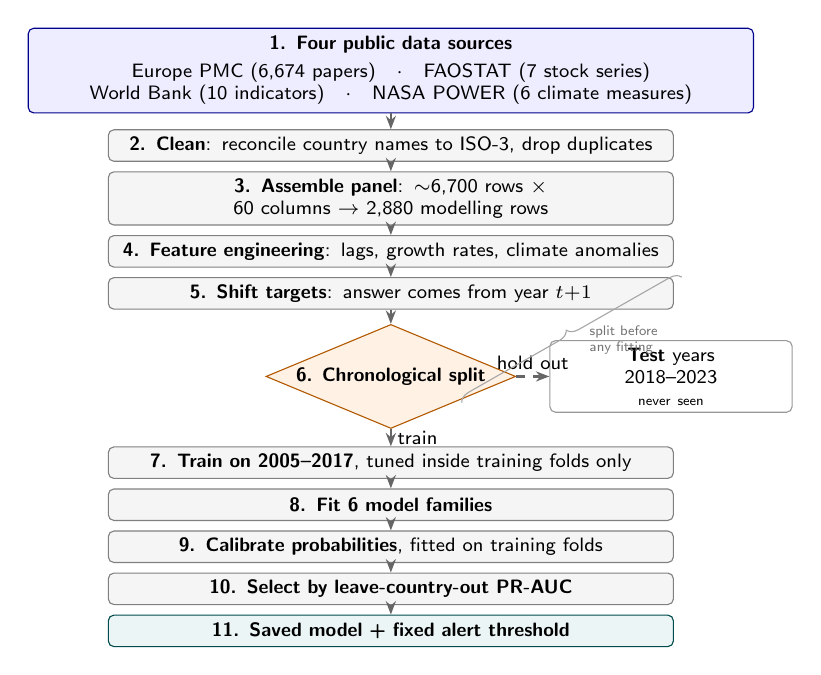
\begin{tikzpicture}[
  st/.style={rectangle,rounded corners=2pt,draw=black!50,fill=black!4,
             align=center,minimum height=0.40cm,text width=7.0cm,
             font=\scriptsize\sffamily,inner sep=2.5pt},
  srcbox/.style={rectangle,rounded corners=2pt,draw=blue!55!black,fill=blue!7,
             align=center,minimum height=0.80cm,text width=9.0cm,
             font=\scriptsize\sffamily,inner sep=3pt},
  dec/.style={diamond,draw=orange!70!black,fill=orange!10,aspect=2.4,
              align=center,font=\scriptsize\sffamily,inner sep=1pt},
  final/.style={rectangle,rounded corners=2pt,draw=teal!60!black,fill=teal!8,
             align=center,minimum height=0.40cm,text width=7.0cm,
             font=\scriptsize\sffamily,inner sep=2.5pt},
  testb/.style={rectangle,rounded corners=2pt,draw=black!40,fill=white,
             align=center,minimum height=0.52cm,text width=2.9cm,
             font=\scriptsize\sffamily,inner sep=2.5pt},
  fl/.style={-{Stealth[length=1.7mm]},thick,draw=black!60},
  step/.style={font=\scriptsize\sffamily\bfseries,text=black!45,anchor=east},
]

  \node[srcbox] (src) at (0,0)
    {\textbf{1. Four public data sources}\\[2pt]
     Europe PMC (6{,}674 papers)\quad$\cdot$\quad FAOSTAT (7 stock series)\\
     World Bank (10 indicators)\quad$\cdot$\quad NASA POWER (6 climate measures)};

  \node[st,below=0.20cm of src] (clean) {\textbf{2. Clean}: reconcile country names to ISO-3, drop duplicates};
  \node[st,below=0.12cm of clean] (panel) {\textbf{3. Assemble panel}: $\sim$6{,}700 rows $\times$ 60 columns $\rightarrow$ 2{,}880 modelling rows};
  \node[st,below=0.12cm of panel] (feat) {\textbf{4. Feature engineering}: lags, growth rates, climate anomalies};
  \node[st,below=0.12cm of feat] (shift) {\textbf{5. Shift targets}: answer comes from year $t{+}1$};
  \node[dec,below=0.18cm of shift] (split) {\textbf{6. Chronological split}};

  % training branch (down)
  \node[st,below=0.22cm of split] (train) {\textbf{7. Train on 2005--2017}, tuned inside training folds only};
  \node[st,below=0.12cm of train] (fit) {\textbf{8. Fit 6 model families}};
  \node[st,below=0.12cm of fit] (cal) {\textbf{9. Calibrate probabilities}, fitted on training folds};
  \node[st,below=0.12cm of cal] (sel) {\textbf{10. Select by leave-country-out PR-AUC}};
  \node[final,below=0.12cm of sel] (saved) {\textbf{11. Saved model + fixed alert threshold}};

  % test branch (right)
  \node[testb,right=0.42cm of split] (test) {\textbf{Test} years\\2018--2023\\\tiny never seen};

  \draw[fl] (src) -- (clean);
  \draw[fl] (clean) -- (panel);
  \draw[fl] (panel) -- (feat);
  \draw[fl] (feat) -- (shift);
  \draw[fl] (shift) -- (split);
  \draw[fl] (split) -- node[font=\scriptsize\sffamily,right=1pt,inner sep=1pt] {train} (train);
  \draw[fl] (train) -- (fit);
  \draw[fl] (fit) -- (cal);
  \draw[fl] (cal) -- (sel);
  \draw[fl] (sel) -- (saved);
  \draw[fl,dashed] (split.east) -- node[font=\scriptsize\sffamily,above,inner sep=2pt] {hold out} (test.west);

  % brace showing where leakage protection sits
  \draw[decorate,decoration={brace,amplitude=4pt,mirror},black!35]
       ([xshift=0.10cm]shift.north east) -- ([xshift=0.10cm]split.south east)
       node[midway,right=3pt,font=\tiny\sffamily,text=black!55,align=left]
       {split before\\any fitting};
\end{tikzpicture}
\caption{Training pipeline. The chronological split sits before any model sees the
data, so the 2018--2023 years never influence training. Tuning and calibration both
happen strictly inside the training years.}
\label{fig:trainflow}
\end{figure}

\begin{figure}[htbp]
\centering
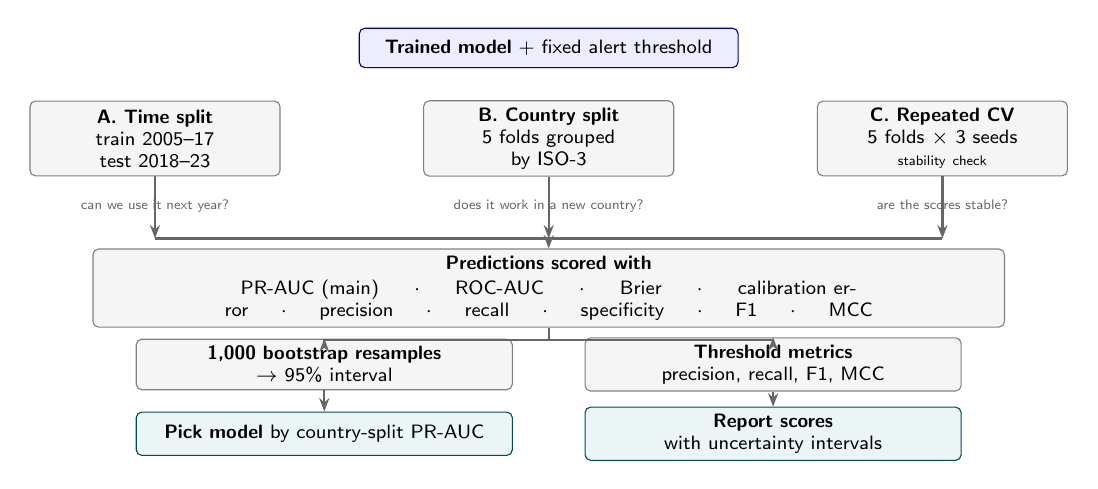
\begin{tikzpicture}[
  bx/.style={rectangle,rounded corners=2pt,draw=black!50,fill=black!4,
             align=center,font=\scriptsize\sffamily,inner sep=2.5pt},
  top/.style={rectangle,rounded corners=2pt,draw=blue!55!black,fill=blue!7,
             align=center,font=\scriptsize\sffamily,inner sep=3pt},
  fin/.style={rectangle,rounded corners=2pt,draw=teal!60!black,fill=teal!8,
             align=center,font=\scriptsize\sffamily,inner sep=2.5pt},
  fl/.style={-{Stealth[length=1.7mm]},thick,draw=black!60},
]

  \node[top,text width=4.6cm,minimum height=0.5cm] (m) at (0,0)
       {\textbf{Trained model} + fixed alert threshold};

  % three schemes
  \node[bx,text width=3.0cm,minimum height=0.95cm] (s1) at (-5.0,-1.15)
       {\textbf{A. Time split}\\train 2005--17\\test 2018--23};
  \node[bx,text width=3.0cm,minimum height=0.95cm] (s2) at (0,-1.15)
       {\textbf{B. Country split}\\5 folds grouped\\by ISO-3};
  \node[bx,text width=3.0cm,minimum height=0.95cm] (s3) at (5.0,-1.15)
       {\textbf{C. Repeated CV}\\5 folds $\times$ 3 seeds\\\tiny stability check};

  \node[font=\tiny\sffamily,text=black!60,anchor=north,text width=3.0cm,align=center] (q1)
       at (-5.0,-1.80) {can we use it next year?};
  \node[font=\tiny\sffamily,text=black!60,anchor=north,text width=3.0cm,align=center] (q2)
       at (0,-1.80) {does it work in a new country?};
  \node[font=\tiny\sffamily,text=black!60,anchor=north,text width=3.0cm,align=center] (q3)
       at (5.0,-1.80) {are the scores stable?};

  % collector rail
  \coordinate (railL) at (-5.0,-2.42);
  \coordinate (railR) at (5.0,-2.42);
  \draw[fl] (s1.south) -- (railL);
  \draw[fl] (s2.south) -- (0,-2.42);
  \draw[fl] (s3.south) -- (railR);
  \draw[thick,draw=black!60] (railL) -- (railR);

  \node[bx,text width=11.4cm,minimum height=0.78cm] (met) at (0,-3.05)
       {\textbf{Predictions scored with}\\[1pt]
        PR-AUC (main) $\;\cdot\;$ ROC-AUC $\;\cdot\;$ Brier $\;\cdot\;$ calibration error
        $\;\cdot\;$ precision $\;\cdot\;$ recall $\;\cdot\;$ specificity $\;\cdot\;$ F1
        $\;\cdot\;$ MCC};
  \draw[fl] (0,-2.42) -- (met.north);

  \node[bx,text width=4.6cm,minimum height=0.62cm] (boot) at (-2.85,-4.02)
       {\textbf{1{,}000 bootstrap resamples}\\$\rightarrow$ 95\% interval};
  \node[bx,text width=4.6cm,minimum height=0.62cm] (alert) at (2.85,-4.02)
       {\textbf{Threshold metrics}\\precision, recall, F1, MCC};

  \node[fin,text width=4.6cm,minimum height=0.55cm] (pick) at (-2.85,-4.90)
       {\textbf{Pick model} by country-split PR-AUC};
  \node[fin,text width=4.6cm,minimum height=0.55cm] (sub) at (2.85,-4.90)
       {\textbf{Report scores}\\with uncertainty intervals};

  \draw[fl] (met.south) -- ++(0,-0.16) -| (boot.north);
  \draw[fl] (met.south) -- ++(0,-0.16) -| (alert.north);
  \draw[fl] (boot) -- (pick);
  \draw[fl] (alert) -- (sub);

\end{tikzpicture}
\caption{Evaluation pipeline. One trained model is scored three different ways, each
answering a different question, then reported with uncertainty intervals.}
\label{fig:evalflow}
\end{figure}


Three schemes answer different questions. A temporal holdout trains on 2005 to 2017 (about 68\% of
rows) and tests on 2018 to 2023 (about 32\%), asking whether the model can be used in following
years. Leave-country-out uses five folds grouped by country, so every prediction is for an unseen
country; that is the harsher test and the one that governs selection. Repeated stratified
cross-validation (five folds, three repeats) is a stability check. A random row split would let the
model memorise country identity, which is why splits are grouped \cite{roberts2017}.

Precision-recall AUC is the primary metric: at 5.87\% prevalence, ROC-AUC is dominated by the
true-negative mass and overstates performance \cite{saito2015,davis2006}, so ROC-AUC is reported only
for comparability. Brier score and expected calibration error check whether predicted probabilities
can support a threshold-based alert \cite{niculescu2005,huang2020}. Precision, recall, specificity,
F1 and Matthews correlation use a threshold tuned on training data only, with bootstrap percentile
intervals over one thousand resamples.

\paragraph{Leakage controls.}
Features use year $t$ or earlier and only the target uses $t{+}1$; the split is chronological;
hyperparameters are tuned inside training folds; calibration is fitted on training folds only; the
alert threshold is fixed on training; and imputation values and missing indicators are generated
inside the pipeline.

\paragraph{Why PR-AUC, calibration and SHAP.}
PR-AUC asks how quickly ranking the riskiest rows surfaces real events; a method with no skill scores
the prevalence (0.0587 here). Calibration groups predictions into buckets and compares each bucket's
average prediction with how often the event happened; the averaged gap is expected calibration error.
SHAP assigns each input a fair share of one prediction by averaging marginal contributions over
feature orderings \cite{lundberg2017}: the values sum to the gap between the base rate and that
prediction, which is why the same numbers support both global feature ranking and the per-prediction
factor list the risk engine returns.

% =====================================================================
\section{Retrieval-Augmented Question Answering}
\label{ch:rag}
% =====================================================================

\subsection{The Problem This Layer Solves}

A calibrated probability of 0.24 is useful to a veterinary officer and opaque to most equine owners,
yet both still have questions that the risk score does not answer: what the National Action Plan
requires, how movement control works, what to do if an animal looks sick, and whether a claim is
still current guidance. Asking a large language model directly is the obvious shortcut and a real
hazard, since a model asked about glanders may answer from outdated training data, conflate glanders
with melioidosis, or invent a treatment protocol, and for a zoonosis under statutory control an
invented instruction is worse than no answer. Retrieval-augmented generation \cite{lewis2020}
restricts what the model may use: it receives a small set of passages from official guidance and,
when relevant, the current prediction's numbers, and must answer only from those passages, so each
claim traces to text the reader can check.

The goal is narrow and testable: answers a veterinary officer would accept as consistent with the
National Action Plan, and a refusal rather than a guess when the corpus does not support one.
Fine-tuning would give fluent text without citations, no clean line between guidance and the base
model's priors, and knowledge frozen at training time, whereas retrieval keeps knowledge in a corpus
that a re-ingestion can update, makes every answer auditable, and allows a refusal path, at the cost
of latency and possible retrieval failure.

\subsection{Knowledge Base}

The corpus is restricted to authoritative sources so that answers can be checked against them, and
each document carries an authority tier used as a tie-breaker during retrieval.

\begin{table}[htbp]
\centering
\caption{Knowledge base, by authority tier.}
\label{tab:corpus}
\small
\begin{tabular}{@{}>{\raggedright\arraybackslash}p{5.0cm}>{\raggedright\arraybackslash}p{1.6cm}>{\raggedright\arraybackslash}p{7.0cm}@{}}
\toprule
\textbf{Source} & \textbf{Tier} & \textbf{Use} \\
\midrule
DAHD National Action Plan for Glanders, 2025 \cite{dahd2025} & 1 & Case definitions, surveillance obligations, movement control, quarantine, notification duties. \\
WOAH and WHO disease information sheets & 1 & Disease biology, transmission, zoonotic risk, official status. \\
ICAR and national laboratory guidance & 2 & Diagnostic sampling, laboratory referral. \\
Open-access publications & 3 & Epidemiology, risk factors, regional situation. \\
\bottomrule
\end{tabular}
\end{table}

Tier 3 may inform an answer but never overrides tier 1 on a control instruction. Conflicts
resolve to the higher tier and are logged, because a silent contradiction between sources is the
failure this layer exists to prevent.

\subsection{Ingestion, Embedding and Retrieval}

Ingestion runs offline as a job and stores each chunk with enough metadata to be cited and filtered.
Chunking is section-aware rather than fixed-width, because a fixed window cuts control instructions in
half and lets the model complete a truncated sentence. The splitter respects headings first, then
paragraphs, falling back to a sliding window only past the ceiling. Chunks target 400 to 700 tokens
with 15 per cent overlap inside a section, and sections under 80 tokens merge into the parent. The
full section path is retained, for example \texttt{NAP-2025 > 5.2 Movement control}, so a citation
points to a subsection rather than a 90-page document.

Chunks are embedded with a compact sentence-transformer \cite{reimers2019} producing 384-dimensional
vectors, with a multilingual variant for Hindi because an English-only embedding degrades on
Devanagari. Vectors live in pgvector beside the relational tables, so re-ingestion and prediction share
one transaction boundary. The index is HNSW with cosine distance \cite{malkov2020}; the reranker
corrects recall at the head of the list, and the index keeps query cost flat as the corpus grows.


\begin{figure}[htbp]
\centering
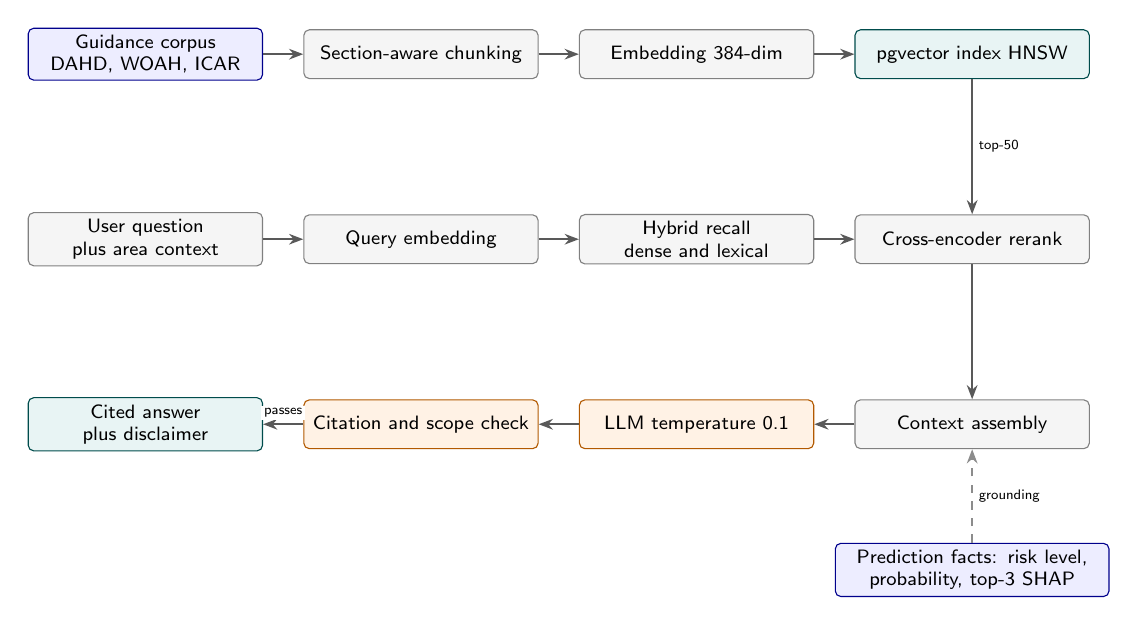
\begin{tikzpicture}[
  st/.style={rectangle,rounded corners=2pt,draw=black!50,fill=black!4,
             align=center,minimum height=0.62cm,text width=2.8cm,
             font=\scriptsize\sffamily,inner sep=2.5pt},
  doc/.style={rectangle,rounded corners=2pt,draw=blue!55!black,fill=blue!7,
              align=center,minimum height=0.62cm,text width=2.8cm,
              font=\scriptsize\sffamily,inner sep=2.5pt},
  gate/.style={rectangle,rounded corners=2pt,draw=orange!70!black,fill=orange!10,
               align=center,minimum height=0.62cm,text width=2.8cm,
               font=\scriptsize\sffamily,inner sep=2.5pt},
  emit/.style={rectangle,rounded corners=2pt,draw=teal!60!black,fill=teal!9,
               align=center,minimum height=0.62cm,text width=2.8cm,
               font=\scriptsize\sffamily,inner sep=2.5pt},
  fl/.style={-{Stealth[length=1.8mm]},thick,draw=black!65},
  dfl/.style={-{Stealth[length=1.8mm]},thick,dashed,draw=black!45},
  l/.style={font=\tiny\sffamily,fill=white,inner sep=1pt,align=center},
]
  % ---- offline ingestion, row 1 -----------------------------------------
  \node[doc] (corpus) at (0,0)      {Guidance corpus\ DAHD, WOAH, ICAR};
  \node[st]  (parse)  at (3.5,0)    {Section-aware\ chunking};
  \node[st]  (emb)    at (7.0,0)    {Embedding\ 384-dim};
  \node[emit] (idx)   at (10.5,0)   {pgvector index\ HNSW};

  % ---- online retrieval, row 2 ------------------------------------------
  \node[st] (q)   at (0,-2.35)   {User question\ plus area context};
  \node[st] (qe)  at (3.5,-2.35) {Query\ embedding};
  \node[st] (hyb) at (7.0,-2.35) {Hybrid recall\ dense and lexical};
  \node[st] (rr)  at (10.5,-2.35){Cross-encoder\ rerank};

  % ---- assembly and generation, row 3 (right to left) -------------------
  \node[st]   (ctx) at (10.5,-4.70) {Context\ assembly};
  \node[gate] (gen) at (7.0,-4.70)  {LLM\ temperature 0.1};
  \node[gate] (gd)  at (3.5,-4.70)  {Citation and\ scope check};
  \node[emit] (ans) at (0,-4.70)    {Cited answer\ plus disclaimer};

  \node[doc,text width=3.3cm] (facts) at (10.5,-6.55)
    {Prediction facts: risk level,\ probability, top-3 SHAP};

  \draw[fl] (corpus) -- (parse);
  \draw[fl] (parse) -- (emb);
  \draw[fl] (emb) -- (idx);

  \draw[fl] (q) -- (qe);
  \draw[fl] (qe) -- (hyb);
  \draw[fl] (hyb) -- (rr);

  \draw[fl] (idx) -- node[l,right=1pt]{top-50} (rr);
  \draw[fl] (rr) -- (ctx);
  \draw[fl] (ctx) -- (gen);
  \draw[fl] (gen) -- (gd);
  \draw[fl] (gd) -- node[l,above=1pt]{passes} (ans);

  \draw[dfl] (facts) -- node[l,right=1pt]{grounding} (ctx);
\end{tikzpicture}
\caption[RAG layer: ingestion, retrieval, assembly and generation]{The RAG layer. Ingestion (top row) is an offline job; retrieval, assembly and generation
(below) run per request. Predicted risk and SHAP factors are injected as structured facts, so the
answer explains this forecast rather than glanders in general. The citation check sits after
generation and can return a refusal instead of an unsupported answer.}
\label{fig:rag}
\end{figure}


Retrieval is hybrid, because dense and lexical search \cite{robertson2009} fail differently here. A
dense query for ``movement control'' may miss a passage using ``restriction of equid movement'', where
a lexical match succeeds; conversely a lexical query for a rare acronym retrieves noise a dense query
ignores. Both lists are fused by reciprocal rank fusion \cite{cormack2009}, which combines rankings
without requiring comparable scores:

\[
\mathrm{RRF}(d) = \sum_{i \in \{\text{dense},\text{lexical}\}} \frac{1}{k + \mathrm{rank}_i(d)},
\qquad k = 60
\]

The fused top fifty are reranked by a cross-encoder scoring each passage against the question
jointly. It is far slower per pair than an embedding dot product, which is why it runs on fifty
candidates rather than the corpus, and the top five become the context.

\begin{table}[htbp]
\centering
\caption{Retrieval parameters.}
\label{tab:retrieval}
\small
\begin{tabular}{@{}lll@{}}
\toprule
\textbf{Stage} & \textbf{Setting} & \textbf{Reason} \\
\midrule
Dense recall & top 30, cosine & Semantic paraphrase coverage \\
Lexical recall & top 30, BM25 & Exact terms, acronyms, section titles \\
Fusion & reciprocal rank, $k=60$ & Scale-free combination of two rankings \\
Rerank & cross-encoder, top 50 to 5 & Precision at the head of the list \\
Relevance floor & rerank score below 0.30 discarded & Prevents padding the context with weak passages \\
\bottomrule
\end{tabular}
\end{table}

The relevance floor drives the refusal path: if fewer than two passages clear it, the layer returns a
refusal with the SHAP factors, because marginal passages produce a confident answer built on
nothing.

\subsection{Context, Generation and Guardrails}

The prompt has three parts in fixed order: a system instruction, the retrieved passages with
identifiers, and (when supplied) structured prediction facts for the area under discussion. The
prediction block is context for questions about a specific forecast; it is not required for general
guidance questions. Facts are injected as structured data so the model cannot rewrite an association
as a cause. The instruction states four constraints: answer only from the passages, cite every claim,
never diagnose an individual animal, and make clear when a population-level forecast is being
discussed.

Generation uses temperature 0.1 and a bounded output length so that two officers asking the same
question about the same area tend to get the same instruction. The provider sits behind a
single-method interface, so one retrieval, grounding and citation path can serve a local Ollama model
or a hosted API; switching model cannot silently disable the guardrails.

The layer is designed to refuse, and four checks can terminate a response.

\begin{table}[htbp]
\centering
\caption{Guardrails and their failure behaviour.}
\label{tab:guardrails}
\small
\begin{tabular}{@{}>{\raggedright\arraybackslash}p{3.0cm}>{\raggedright\arraybackslash}p{5.2cm}>{\raggedright\arraybackslash}p{5.4cm}@{}}
\toprule
\textbf{Check} & \textbf{What it verifies} & \textbf{On failure} \\
\midrule
Retrieval floor & At least two passages above the relevance threshold & Refusal with the top SHAP factors, which need no retrieval \\
Citation resolution & Every cited identifier exists in the retrieved set & Answer rejected and regenerated once, then refusal \\
Diagnosis scope & No individual-animal diagnosis or treatment prescription & Response rewritten without the clinical claim, and the attempt logged \\
Out-of-scope & Question is about glanders control, not unrelated topics & Refusal stating what the layer covers \\
\bottomrule
\end{tabular}
\end{table}

The citation check is mechanical: the answer is parsed for identifiers and each is looked up in the
retrieved set, and one that does not resolve means the model cited a document it was not given, which
is a hallucination whether or not the sentence is true. Asking a model to be accurate is not a
control; checking its output is.

\subsection{Evaluation}

Five quantities are defined below, following the project proposal. None is reported as a measurement,
because the layer has not been run against the corpus; measuring them is future work
(Chapter~\ref{ch:concl}).

\textbf{Retrieval quality.} Recall@$k$, the fraction of hand-built questions whose known relevant
passage appears in the top $k$ results, at $k=5$, with mean reciprocal rank, which rewards returning it
near the top rather than merely inside the cut-off. This isolates retrieval from generation, since no
generation quality helps if the right passage is never retrieved.

\textbf{Faithfulness.} The fraction of claims the retrieved context supports, scored by a judge model
and reviewed by hand on a sample; the RAGAS-style metric that catches a model citing a passage while
saying something the passage does not say.

\textbf{Answer relevance.} Whether the answer addresses the question asked rather than reciting
correct but tangential guidance, scored on the same sample, since an answer can be grounded and still
unhelpful.

\textbf{Citation precision.} The fraction of citations resolving to a passage that supports the
sentence, distinct from resolution, which only checks existence.

\textbf{Refusal behaviour.} The refusal rate on out-of-scope questions and the false refusal rate in
scope: a layer that never refuses is unsafe and one that always refuses is useless.

Deployment targets, so the claim is falsifiable: recall@5 above 0.85, faithfulness and answer
relevance above 0.90 and 0.85, citation precision above 0.95, a false refusal rate below 10 per cent,
and p95 latency under two seconds.

% =====================================================================
% GlandersWatch Technical Writing Report — Alerting System chapter
%
%
% The two supplied standalone TikZ diagrams must remain in:
%   figures/alerts_pipeline.tex
%   figures/alerting_modular_arch.tex
% =====================================================================

\section{Alerting System}
\label{ch:alerts}

\subsection{Purpose and Scope}
The GlandersWatch alerting system converts a machine-learning risk prediction into a controlled notification for registered recipients. The risk engine estimates the probability of documented Glanders occurrence for an area and period; the alert service decides whether to notify, who should receive the message and how delivery is managed. A prediction is not itself an alert: every new prediction is evaluated, but a notification is generated only when the configured policy requires it.

The design is period-aware and uses one workflow for monthly and yearly predictions. Monthly prediction is future work for the ML component; the currently evaluated model is country-year based. The alert service is designed to accept monthly records once a monthly model, target and data pipeline have been developed and validated. Its output is a population-level warning, not an individual-animal diagnosis or a replacement for veterinary examination and laboratory testing.

Related warning systems, design lessons and the comparison with this service are reviewed in
Chapter~\ref{ch:lit} (Tables~\ref{tab:alert-related-work} and~\ref{tab:alert-comparison}). This
section specifies the architecture and rules that implement that design.

\subsection{Proposed End-to-End Architecture}
Figure~\ref{fig:alerts-pipeline} shows the supplied end-to-end architecture. The flow begins with user registration and prediction generation, then proceeds through evaluation, rules, alert creation, fan-out and notification. The data layer stores predictions, subscriptions, period-specific alert state, alerts and delivery logs. The approval gate is optional and may hold selected HIGH alerts for veterinary review; its use requires agreement with project and veterinary stakeholders.

\begin{figure}[htbp]\centering
\resizebox{\textwidth}{!}{\documentclass[tikz,border=10pt]{standalone}
\usepackage[T1]{fontenc}
\usepackage[scaled=0.95]{helvet}
\renewcommand{\familydefault}{\sfdefault}
\usepackage{xcolor}
\usetikzlibrary{arrows.meta,shapes.geometric,calc}

% ---------- palette ----------
\definecolor{gwnavy}{HTML}{1F3A5F}
\definecolor{gwteal}{HTML}{0F766E}
\definecolor{gwamber}{HTML}{B45309}
\definecolor{gwgreen}{HTML}{15803D}
\definecolor{gwslate}{HTML}{475569}
\definecolor{gwviolet}{HTML}{6D28D9}
\definecolor{gwblue}{HTML}{1D4ED8}

% ---------- step badge ----------
\newcommand{\sn}[1]{\tikz[baseline=(c.base)]\node[circle,fill=gwnavy,text=white,inner sep=0pt,minimum size=0.36cm,text width=0.36cm,align=center,font=\bfseries\scriptsize](c){#1};}

% ---------- styles ----------
\tikzset{
  box/.style={draw=#1!75!black, fill=#1!7, rounded corners=3pt, line width=0.8pt, align=left, font=\small},
  flow/.style={-{Stealth[length=2.6mm,width=2mm]}, line width=1.1pt, gwnavy},
  dbw/.style={-{Stealth[length=2.2mm,width=1.7mm]}, dashed, line width=0.8pt, gwslate},
  dbr/.style={{Stealth[length=2.2mm,width=1.7mm]}-, dashed, line width=0.8pt, gwslate},
  dbrw/.style={{Stealth[length=2.2mm,width=1.7mm]}-{Stealth[length=2.2mm,width=1.7mm]}, dashed, line width=0.8pt, gwslate},
  opt/.style={{Stealth[length=2.2mm,width=1.7mm]}-{Stealth[length=2.2mm,width=1.7mm]}, dashed, line width=0.9pt, gwviolet},
  lbl/.style={font=\scriptsize\bfseries, text=gwnavy, fill=white, inner sep=1.2pt},
  lbls/.style={font=\scriptsize, text=gwslate, inner sep=1pt},
}

% \blk{name}{color}{x1}{y1}{x2}{y2}{extra}{text}
\newcommand{\blk}[8]{%
  \pgfmathsetlengthmacro{\bw}{(#5-#3)*1cm}%
  \pgfmathsetlengthmacro{\bh}{(#6-#4)*1cm}%
  \pgfmathsetlengthmacro{\tw}{(#5-#3)*1cm-10pt}%
  \node[box=#2,#7,anchor=south west,minimum width=\bw,minimum height=\bh,text width=\tw,inner sep=5pt](#1) at (#3,#4){#8};}

% \cont{color}{x1}{y1}{x2}{y2}{title}
\newcommand{\cont}[6]{%
  \draw[draw=#1!70!black, fill=#1!4, rounded corners=5pt, line width=1pt] (#2,#3) rectangle (#4,#5);
  \node[anchor=north west, font=\small\bfseries, text=#1!60!black] at (#2+0.2,#5-0.12) {#6};}

\begin{document}
\begin{tikzpicture}[x=1cm,y=1cm]

% ================= TITLE =================
\node[anchor=west, font=\Large\bfseries, text=gwnavy] at (0.4,18.9) {GlandersWatch --- Alerting System Architecture};
\node[anchor=west, font=\small, text=gwslate] at (0.4,18.25) {From a calibrated risk probability to a message in an owner's hand: threshold $\rightarrow$ suppression $\rightarrow$ deduplication $\rightarrow$ notification};

% ================= TOP LANE =================

\blk{intake}{gwblue}{0.4}{15.2}{9.4}{17.6}{}{\textbf{\sn{S}\ User registration} \textit{(once, with the app)}\\[2pt]
Next.js form $\rightarrow$ FastAPI \texttt{POST /register} (JWT)\\
phone OTP $\cdot$ consent $\cdot$ area $\cdot$ language\\
registered = enrolled for alerts; \texttt{STOP} opts out}

\blk{p1}{gwslate}{10.8}{15.2}{15.4}{17.6}{}{\textbf{Forecast only}\\[2pt]Every message states it is a population-level forecast, never a diagnosis.}
\blk{p2}{gwslate}{15.6}{15.2}{20.2}{17.6}{}{\textbf{Idempotent}\\[2pt]Every step is safe to retry: no job, restart or retrain can send twice.}
\blk{p3}{gwslate}{20.4}{15.2}{25.0}{17.6}{}{\textbf{Configurable}\\[2pt]Cut-offs, cooldowns and quiet hours live in the DB, editable by an admin.}
\blk{p4}{gwslate}{25.2}{15.2}{29.8}{17.6}{}{\textbf{Auditable}\\[2pt]Every decision (sent or skipped) is logged with a reason code.}

% ================= MAIN BAND =================
\blk{trig}{gwteal}{0.4}{9.8}{3.9}{13.8}{}{\textbf{\sn{1}\ Trigger}\\[2pt]
ML risk-engine job\\
Celery beat, once per prediction period\\[2pt]
writes \texttt{predictions}\\
\textit{(area, period, p, model\_ver)}\\
then emits \textit{predictions\_ready}}

\blk{eval}{gwteal}{5.6}{9.0}{9.4}{13.8}{}{\textbf{\sn{2}\ Alert Evaluator}\\[2pt]
Celery worker, wakes on the event.\\[2pt]
For every area with registered users:\\
$\bullet$ load latest probability $p$\\
$\bullet$ load previous alert level\\
$\bullet$ hand $(area,\,p,\,prev)$ to the rules\\[2pt]
Areas with no registered users are skipped.}

% ---- rules engine ----
\cont{gwamber}{10.8}{5.5}{17.8}{14.5}{\sn{3}\ Rules Engine --- decides whether to send}
\blk{rA}{gwamber}{11.1}{11.7}{17.5}{13.8}{}{\textbf{A\ \ Threshold}\\[2pt]
calibrated $p \rightarrow$ LOW / MEDIUM / HIGH\\
cut-offs configurable (set from validation results)\\
hysteresis: leave HIGH only when $p < T-\delta$}
\blk{rB}{gwamber}{11.1}{8.8}{17.5}{11.25}{}{\textbf{B\ \ Suppression}\\[2pt]
send only on a level change (e.g.\ MEDIUM $\rightarrow$ HIGH)\\
cooldown per area + level; escalation bypasses it\\
per-user daily cap $\cdot$ quiet hours\\
stale-data guard $\cdot$ admin mute}
\blk{rC}{gwamber}{11.1}{6.2}{17.5}{8.35}{}{\textbf{C\ \ Deduplication}\\[2pt]
key = (area, period, level), UNIQUE in DB\\
per-recipient key = (alert, user)\\
re-check delivery log before every send / retry}
\draw[flow] (14.3,11.7) -- (14.3,11.25);
\draw[flow] (14.3,8.8) -- (14.3,8.35);

% ---- alert record + optional gate ----
\blk{rec}{gwgreen}{19.0}{11.7}{22.6}{14.4}{}{\textbf{\sn{4}\ Alert record}\\[2pt]
row in \texttt{alerts}\\
status: pending $\rightarrow$ queued\\
$\rightarrow$ sent / failed}
\blk{gate}{gwviolet}{19.0}{6.4}{22.6}{9.0}{dashed}{\textbf{Optional approval gate}\\[2pt]
HIGH alerts held for a veterinary officer, then released}

% ---- right column ----
\blk{que}{gwgreen}{24.2}{12.6}{29.8}{14.4}{}{\textbf{\sn{5}\ Fan-out queue} (Redis)\\[2pt]
one job per registered user, each idempotent}

\cont{gwgreen}{24.2}{4.0}{29.8}{11.6}{\sn{6}\ Notification Service}
\blk{ren}{gwgreen}{24.5}{8.7}{29.5}{10.5}{}{\textbf{Template renderer}\\
user's language (EN / HI) $\cdot$ fixed templates\\
risk + action + vet contact + disclaimer}
\draw[box=gwgreen, rounded corners=3pt, line width=0.8pt] (24.5,6.4) rectangle (29.5,8.4);
\node[anchor=north west, font=\small\bfseries, text=black] at (24.6,8.35) {Channel adapters};
\foreach \x/\t in {24.65/SMS,26.2/WhatsApp,27.75/Telegram$^{*}$}{
  \node[draw=gwgreen!70!black, fill=white, rounded corners=2pt, font=\scriptsize\bfseries, minimum width=1.5cm, minimum height=0.55cm, anchor=south west, inner sep=1pt] at (\x,6.55) {\t};}
\blk{ret}{gwgreen}{24.5}{4.5}{29.5}{6.2}{}{\textbf{Retry + backoff}\\
fallback channel on failure; status via \mbox{webhooks}}

\blk{rcp}{gwnavy}{24.2}{0.5}{29.8}{2.9}{}{\textbf{\sn{7}\ Owner / field worker}\\[2pt]
Risk level + short preventive action + veterinary contact.\\
\textit{``Population-level forecast, not a diagnosis.''}}

% ================= DATA LAYER =================
\draw[draw=gwslate!70!black, fill=gwslate!6, rounded corners=5pt, line width=1pt] (0.4,0.5) rectangle (17.8,3.7);
\node[anchor=north west, font=\small\bfseries, text=gwslate!80!black] at (0.6,3.62) {Data layer --- PostgreSQL / PostGIS};
\foreach \c/\n/\d in {2.1/predictions/{from ML},5.55/users/{phone, area, language},9.0/alert\_state/{last level, last sent},12.45/alerts/{+ decision log},15.9/delivery\_logs/{per message}}{
  \draw[draw=gwslate!75!black, fill=white, line width=0.8pt] (\c-1.4,0.75) -- (\c-1.4,2.5) arc (180:360:1.4 and 0.22) -- (\c+1.4,0.75) arc (360:180:1.4 and 0.22);
  \draw[draw=gwslate!75!black, fill=gwslate!8, line width=0.8pt] (\c,2.5) ellipse (1.4 and 0.22);
  \node[font=\scriptsize\bfseries\ttfamily, text=black] at (\c,1.75) {\n};
  \node[font=\scriptsize, text=gwslate] at (\c,1.25) {\d};
}

\blk{adm}{gwblue}{19.0}{0.5}{22.6}{3.4}{}{\textbf{Admin dashboard}\\[1pt]
Next.js\\
alert history $\cdot$ delivery status\\
mute / override $\cdot$ approvals}

% ================= ARROWS =================
% setup path
\draw[flow] (7.5,15.2) -- (7.5,13.8) node[midway,right,lbls]{registered users};
% trigger -> evaluator -> rules
\draw[flow] (3.9,12.3) -- (5.6,12.3) node[midway,above,lbl]{event};
\draw[flow] (9.4,12.3) -- (10.8,12.3) node[midway,above,lbl]{$p$, prev};
% SEND path
\draw[flow, rounded corners=4pt] (17.5,7.3) -- (18.4,7.3) -- (18.4,13.0) -- (19.0,13.0);
\node[lbl, rotate=90] at (18.4,10.2) {SEND};
% record -> queue -> service -> recipient
\draw[flow] (22.6,13.0) -- (24.2,13.0);
\draw[flow] (27.0,12.6) -- (27.0,11.6);
\draw[flow] (27.0,4.0) -- (27.0,2.9);
% optional gate
\draw[opt] (20.8,11.7) -- (20.8,9.0) node[midway,right,lbls,text=gwviolet]{HIGH only};
\draw[opt] (19.5,6.4) -- (19.5,3.4) node[pos=0.45,right,lbls,text=gwviolet]{approve / reject};
% database arrows
\draw[dbw] (2.15,9.8) -- (2.15,3.7) node[midway,right,lbls]{writes predictions};
\draw[dbr] (7.5,9.0) -- (7.5,3.7) node[pos=0.5,right,lbls,text width=2.6cm,align=left]{reads: predictions, users, alert\_state};
\draw[dbw] (14.3,5.5) -- (14.3,3.7) node[midway,left,lbls]{every decision logged with reason};
\draw[dbw, rounded corners=3pt] (24.2,4.3) -- (15.9,4.3) -- (15.9,3.7);
\node[lbls, anchor=south] at (21.5,4.3) {delivery status webhooks};
\draw[dbrw] (17.8,2.0) -- (19.0,2.0);

% ================= LEGEND =================
\draw[flow] (0.4,-0.5) -- (1.6,-0.5);
\node[anchor=west, font=\scriptsize] at (1.7,-0.5) {control / data flow};
\draw[dbw] (5.2,-0.5) -- (6.4,-0.5);
\node[anchor=west, font=\scriptsize] at (6.5,-0.5) {database read / write};
\draw[opt] (10.4,-0.5) -- (11.6,-0.5);
\node[anchor=west, font=\scriptsize] at (11.7,-0.5) {optional step, to be confirmed with the professor};
\node[anchor=west, font=\scriptsize] at (19.0,-0.5) {$^{*}$ Telegram used for the free demo; SMS / WhatsApp for production (DLT / template approval needed in India)};

\end{tikzpicture}
\end{document}

% \documentclass[tikz,border=10pt]{standalone}
% \usepackage[T1]{fontenc}
% \usepackage[scaled=0.95]{helvet}
% \renewcommand{\familydefault}{\sfdefault}
% \usepackage{xcolor}
% \usetikzlibrary{arrows.meta,shapes.geometric,calc}

% % ---------- palette ----------
% \definecolor{gwnavy}{HTML}{1F3A5F}
% \definecolor{gwteal}{HTML}{0F766E}
% \definecolor{gwamber}{HTML}{B45309}
% \definecolor{gwgreen}{HTML}{15803D}
% \definecolor{gwslate}{HTML}{475569}
% \definecolor{gwviolet}{HTML}{6D28D9}
% \definecolor{gwblue}{HTML}{1D4ED8}

% % ---------- step badge ----------
% \newcommand{\sn}[1]{\tikz[baseline=(c.base)]\node[circle,fill=gwnavy,text=white,inner sep=0pt,minimum size=0.36cm,text width=0.36cm,align=center,font=\bfseries\tiny](c){#1};}

% % ---------- styles ----------
% \tikzset{
%   box/.style={draw=#1!75!black, fill=#1!7, rounded corners=3pt, line width=0.8pt, align=left, font=\scriptsize},
%   flow/.style={-{Stealth[length=2.6mm,width=2mm]}, line width=1.1pt, gwnavy},
%   dbw/.style={-{Stealth[length=2.2mm,width=1.7mm]}, dashed, line width=0.8pt, gwslate},
%   dbr/.style={{Stealth[length=2.2mm,width=1.7mm]}-, dashed, line width=0.8pt, gwslate},
%   dbrw/.style={{Stealth[length=2.2mm,width=1.7mm]}-{Stealth[length=2.2mm,width=1.7mm]}, dashed, line width=0.8pt, gwslate},
%   opt/.style={{Stealth[length=2.2mm,width=1.7mm]}-{Stealth[length=2.2mm,width=1.7mm]}, dashed, line width=0.9pt, gwviolet},
%   lbl/.style={font=\tiny\bfseries, text=gwnavy, fill=white, inner sep=1.2pt},
%   lbls/.style={font=\tiny, text=gwslate, inner sep=1pt},
% }

% % \blk{name}{color}{x1}{y1}{x2}{y2}{extra}{text}
% \newcommand{\blk}[8]{%
%   \pgfmathsetlengthmacro{\bw}{(#5-#3)*1cm}%
%   \pgfmathsetlengthmacro{\bh}{(#6-#4)*1cm}%
%   \pgfmathsetlengthmacro{\tw}{(#5-#3)*1cm-10pt}%
%   \node[box=#2,#7,anchor=south west,minimum width=\bw,minimum height=\bh,text width=\tw,inner sep=5pt](#1) at (#3,#4){#8};}

% % \cont{color}{x1}{y1}{x2}{y2}{title}
% \newcommand{\cont}[6]{%
%   \draw[draw=#1!70!black, fill=#1!4, rounded corners=5pt, line width=1pt] (#2,#3) rectangle (#4,#5);
%   \node[anchor=north west, font=\small\bfseries, text=#1!60!black] at (#2+0.2,#5-0.12) {#6};}

% \begin{document}
% \begin{tikzpicture}[x=1cm,y=1cm]

% % ================= TITLE =================
% \node[anchor=west, font=\Large\bfseries, text=gwnavy] at (0.4,18.9) {GlandersWatch --- Alerting System Architecture};
% \node[anchor=west, font=\small, text=gwslate] at (0.4,18.25) {From a calibrated risk probability to a message in an owner's hand: threshold $\rightarrow$ suppression $\rightarrow$ deduplication $\rightarrow$ notification};

% % ================= TOP LANE =================

% \blk{intake}{gwblue}{0.4}{15.2}{9.4}{17.6}{}{\textbf{\sn{S}\ User registration} \textit{(once, with the app)}\\[2pt]
% Next.js form $\rightarrow$ FastAPI \texttt{POST /register} (JWT)\\
% phone OTP $\cdot$ consent $\cdot$ area $\cdot$ language\\
% registered = enrolled for alerts; \texttt{STOP} opts out}

% \blk{p1}{gwslate}{10.8}{15.2}{15.4}{17.6}{}{\textbf{Forecast only}\\[2pt]Every message states it is a population-level forecast, never a diagnosis.}
% \blk{p2}{gwslate}{15.6}{15.2}{20.2}{17.6}{}{\textbf{Idempotent}\\[2pt]Every step is safe to retry: no job, restart or retrain can send twice.}
% \blk{p3}{gwslate}{20.4}{15.2}{25.0}{17.6}{}{\textbf{Configurable}\\[2pt]Cut-offs, cooldowns and quiet hours live in the DB, editable by an admin.}
% \blk{p4}{gwslate}{25.2}{15.2}{29.8}{17.6}{}{\textbf{Auditable}\\[2pt]Every decision (sent or skipped) is logged with a reason code.}

% % ================= MAIN BAND =================
% \blk{trig}{gwteal}{0.4}{9.8}{3.9}{13.8}{}{\textbf{\sn{1}\ Trigger}\\[2pt]
% ML risk-engine job\\
% Celery beat, once per prediction period\\[2pt]
% writes \texttt{predictions}\\
% \textit{(area, period, p, model\_ver)}\\
% then emits \textit{predictions\_ready}}

% \blk{eval}{gwteal}{5.6}{9.0}{9.4}{13.8}{}{\textbf{\sn{2}\ Alert Evaluator}\\[2pt]
% Celery worker, wakes on the event.\\[2pt]
% For every area with registered users:\\
% $\bullet$ load latest probability $p$\\
% $\bullet$ load previous alert level\\
% $\bullet$ hand $(area,\,p,\,prev)$ to the rules\\[2pt]
% Areas with no registered users are skipped.}

% % ---- rules engine ----
% \cont{gwamber}{10.8}{5.5}{17.8}{14.5}{\sn{3}\ Rules Engine --- decides whether to send}
% \blk{rA}{gwamber}{11.1}{11.7}{17.5}{13.8}{}{\textbf{A\ \ Threshold}\\[2pt]
% calibrated $p \rightarrow$ LOW / MEDIUM / HIGH\\
% cut-offs configurable (set from validation results)\\
% hysteresis: leave HIGH only when $p < T-\delta$}
% \blk{rB}{gwamber}{11.1}{8.8}{17.5}{11.25}{}{\textbf{B\ \ Suppression}\\[2pt]
% send only on a level change (e.g.\ MEDIUM $\rightarrow$ HIGH)\\
% cooldown per area + level; escalation bypasses it\\
% per-user daily cap $\cdot$ quiet hours\\
% stale-data guard $\cdot$ admin mute}
% \blk{rC}{gwamber}{11.1}{6.2}{17.5}{8.35}{}{\textbf{C\ \ Deduplication}\\[2pt]
% key = (area, period, level), UNIQUE in DB\\
% per-recipient key = (alert, user)\\
% re-check delivery log before every send / retry}
% \draw[flow] (14.3,11.7) -- (14.3,11.25);
% \draw[flow] (14.3,8.8) -- (14.3,8.35);

% % ---- alert record + optional gate ----
% \blk{rec}{gwgreen}{19.0}{11.7}{22.6}{14.4}{}{\textbf{\sn{4}\ Alert record}\\[2pt]
% row in \texttt{alerts}\\
% status: pending $\rightarrow$ queued\\
% $\rightarrow$ sent / failed}
% \blk{gate}{gwviolet}{19.0}{6.4}{22.6}{9.0}{dashed}{\textbf{Optional approval gate}\\[2pt]
% HIGH alerts held for a veterinary officer, then released}

% % ---- right column ----
% \blk{que}{gwgreen}{24.2}{12.6}{29.8}{14.4}{}{\textbf{\sn{5}\ Fan-out queue} (Redis)\\[2pt]
% one job per registered user, each idempotent}

% \cont{gwgreen}{24.2}{4.0}{29.8}{11.6}{\sn{6}\ Notification Service}
% \blk{ren}{gwgreen}{24.5}{8.7}{29.5}{10.5}{}{\textbf{Template renderer}\\
% user's language (EN / HI) $\cdot$ fixed templates\\
% risk + action + vet contact + disclaimer}
% \draw[box=gwgreen, rounded corners=3pt, line width=0.8pt] (24.5,6.4) rectangle (29.5,8.4);
% \node[anchor=north west, font=\scriptsize\bfseries, text=black] at (24.6,8.35) {Channel adapters};
% \foreach \x/\t in {24.65/SMS,26.2/WhatsApp,27.75/Telegram$^{*}$}{
%   \node[draw=gwgreen!70!black, fill=white, rounded corners=2pt, font=\tiny\bfseries, minimum width=1.5cm, minimum height=0.55cm, anchor=south west, inner sep=1pt] at (\x,6.55) {\t};}
% \blk{ret}{gwgreen}{24.5}{4.5}{29.5}{6.2}{}{\textbf{Retry + backoff}\\
% fallback channel on failure; status via \mbox{webhooks}}

% \blk{rcp}{gwnavy}{24.2}{0.5}{29.8}{2.9}{}{\textbf{\sn{7}\ Owner / field worker}\\[2pt]
% Risk level + short preventive action + veterinary contact.\\
% \textit{``Population-level forecast, not a diagnosis.''}}

% % ================= DATA LAYER =================
% \draw[draw=gwslate!70!black, fill=gwslate!6, rounded corners=5pt, line width=1pt] (0.4,0.5) rectangle (17.8,3.7);
% \node[anchor=north west, font=\small\bfseries, text=gwslate!80!black] at (0.6,3.62) {Data layer --- PostgreSQL / PostGIS};
% \foreach \c/\n/\d in {2.1/predictions/{from ML},5.55/users/{phone, area, language},9.0/alert\_state/{last level, last sent},12.45/alerts/{+ decision log},15.9/delivery\_logs/{per message}}{
%   \draw[draw=gwslate!75!black, fill=white, line width=0.8pt] (\c-1.4,0.75) -- (\c-1.4,2.5) arc (180:360:1.4 and 0.22) -- (\c+1.4,0.75) arc (360:180:1.4 and 0.22);
%   \draw[draw=gwslate!75!black, fill=gwslate!8, line width=0.8pt] (\c,2.5) ellipse (1.4 and 0.22);
%   \node[font=\scriptsize\bfseries\ttfamily, text=black] at (\c,1.75) {\n};
%   \node[font=\tiny, text=gwslate] at (\c,1.25) {\d};
% }

% \blk{adm}{gwblue}{19.0}{0.5}{22.6}{3.4}{}{\textbf{Admin dashboard}\\[1pt]
% Next.js\\
% alert history $\cdot$ delivery status\\
% mute / override $\cdot$ approvals}

% % ================= ARROWS =================
% % setup path
% \draw[flow] (7.5,15.2) -- (7.5,13.8) node[midway,right,lbls]{registered users};
% % trigger -> evaluator -> rules
% \draw[flow] (3.9,12.3) -- (5.6,12.3) node[midway,above,lbl]{event};
% \draw[flow] (9.4,12.3) -- (10.8,12.3) node[midway,above,lbl]{$p$, prev};
% % SEND path
% \draw[flow, rounded corners=4pt] (17.5,7.3) -- (18.4,7.3) -- (18.4,13.0) -- (19.0,13.0);
% \node[lbl, rotate=90] at (18.4,10.2) {SEND};
% % record -> queue -> service -> recipient
% \draw[flow] (22.6,13.0) -- (24.2,13.0);
% \draw[flow] (27.0,12.6) -- (27.0,11.6);
% \draw[flow] (27.0,4.0) -- (27.0,2.9);
% % optional gate
% \draw[opt] (20.8,11.7) -- (20.8,9.0) node[midway,right,lbls,text=gwviolet]{HIGH only};
% \draw[opt] (19.5,6.4) -- (19.5,3.4) node[pos=0.45,right,lbls,text=gwviolet]{approve / reject};
% % database arrows
% \draw[dbw] (2.15,9.8) -- (2.15,3.7) node[midway,right,lbls]{writes predictions};
% \draw[dbr] (7.5,9.0) -- (7.5,3.7) node[pos=0.5,right,lbls,text width=2.6cm,align=left]{reads: predictions, users, alert\_state};
% \draw[dbw] (14.3,5.5) -- (14.3,3.7) node[midway,left,lbls]{every decision logged with reason};
% \draw[dbw, rounded corners=3pt] (24.2,4.3) -- (15.9,4.3) -- (15.9,3.7);
% \node[lbls, anchor=south] at (21.5,4.3) {delivery status webhooks};
% \draw[dbrw] (17.8,2.0) -- (19.0,2.0);

% % ================= LEGEND =================
% \draw[flow] (0.4,-0.5) -- (1.6,-0.5);
% \node[anchor=west, font=\tiny] at (1.7,-0.5) {control / data flow};
% \draw[dbw] (5.2,-0.5) -- (6.4,-0.5);
% \node[anchor=west, font=\tiny] at (6.5,-0.5) {database read / write};
% \draw[opt] (10.4,-0.5) -- (11.6,-0.5);
% \node[anchor=west, font=\tiny] at (11.7,-0.5) {optional step, to be confirmed with the professor};
% \node[anchor=west, font=\tiny] at (19.0,-0.5) {$^{*}$ Telegram used for the free demo; SMS / WhatsApp for production (DLT / template approval needed in India)};

% \end{tikzpicture}
% \end{document}
}
\caption{End-to-end GlandersWatch alert pipeline. The period field supports monthly or yearly predictions.}\label{fig:alerts-pipeline}
\end{figure}

\subsubsection{Prediction Trigger and Alert Evaluator}
After the risk engine stores a prediction, it publishes \texttt{predictions\_ready}, which tells the evaluator that a prediction batch is available without implying that a message must be sent. The evaluator loads the new prediction, previous state for the same area and frequency, active subscriptions and applicable configuration, then passes these inputs to the rules core; it does not train the model or calculate the probability.

\subsubsection{Rules, Alert Record and Fan-Out}
The rules engine classifies the probability, checks suppression conditions and protects alert creation against duplicates. If the decision is SEND, one logical alert record is created with its area, period, level, source prediction, reason and status. This record is separate from delivery jobs: one alert for Area A may generate 41 jobs for 40 owners and one veterinary officer.

Fan-out obtains eligible subscriptions and creates one job per subscription. Redis with Celery is a proposed production option: Redis brokers background work and Celery workers execute it. The queue is not the permanent alert-history store; PostgreSQL is proposed for durable predictions, states, alerts and delivery logs.

\subsubsection{Notification Service, Data and Administration}
For each job, the notification service checks recipient preferences and delivery restrictions, renders an approved template in the recipient's language and submits it through a channel adapter. The design allows SMS, WhatsApp and Telegram, with email or webhook adapters as extensions. Messages should state the area, period and risk level, provide approved action guidance and veterinary contact information where available, and clarify that the result is a population-level forecast, not a diagnosis.

Temporary provider failures may be retried with backoff, while permanent failures such as invalid destinations are recorded without endless retries. PostgreSQL stores predictions, users/subscriptions, alert state, alert records and delivery logs, with PostGIS available if geographic queries are needed, and the admin dashboard exposes alert history, delivery status, mute controls and any approval workflow under permission-controlled, logged administrative actions.

\subsubsection{Notification Content and Recipient Action}
A useful warning should be short enough to read on a phone but contain enough context for the recipient to understand why it was sent. Each message should identify the affected area, prediction period, risk category, issue date and recommended next step. It should avoid technical model terminology and should not present the probability as the chance that a particular animal is infected. The message should also identify the responsible veterinary contact or official information source, where one is available. The language and channel must follow the recipient's saved preferences and consent.

An illustrative message for a HIGH-risk transition is:
\begin{quote}\small
\textbf{GlandersWatch risk alert -- Area A}\\
\textbf{Period:} March 2027\\
\textbf{Risk level:} HIGH\\
The model indicates an elevated area-level risk of documented Glanders occurrence for this period. This is an early-warning signal, not a diagnosis of any animal. Avoid moving or mixing animals suspected of illness, observe for unusual signs and contact your local veterinary officer for guidance. Do not handle suspected cases without appropriate advice.\\
\textit{For assessment and reporting, contact: [local veterinary contact].}
\end{quote}
The exact action wording should be approved by veterinary authorities before deployment and adapted to local language and operating procedures. A message should not disclose another user's contact details or unnecessary personal information. If no verified local contact is configured, the system should direct recipients to an approved general veterinary service rather than inventing a phone number. Message templates should be versioned so the content used for each alert can be reconstructed during an audit.

\subsection{Period-Aware Prediction Contract}
The prediction must identify its frequency and exact period. A conceptual monthly record is shown below; field names are illustrative and can be aligned with the final API schema.
\begin{verbatim}
{
  "area_id": "AREA-A", "period_type": "month",
  "period_id": "2027-03",
  "period_start": "2027-03-01", "period_end": "2027-03-31",
  "probability": 0.34, "model_version": "gw-model-v1.2",
  "data_freshness": {"passes": true}
}
\end{verbatim}
For yearly records, \texttt{period\_type} is \texttt{year} and the period ID identifies the year. The same evaluator and rules core process either type. State is stored separately by area and frequency: a March 2027 monthly result must not overwrite Area A's 2027 yearly state.

A period-aware logical alert key is:
\[
K_{alert}=(\text{area\_id},\text{period\_type},\text{period\_id},\text{risk\_level}).
\]
This prevents a monthly alert from colliding with a yearly alert for the same area. Cooldowns, freshness requirements and thresholds may also be configured by frequency; monthly settings should not simply inherit yearly values without validation.

\begin{table}[htbp]\centering\small
\caption{Monthly and yearly operation in the same alert service.}\label{tab:monthly-yearly}
\begin{tabular}{p{2.7cm}p{5.0cm}p{5.0cm}}\toprule
\textbf{Aspect}&\textbf{Monthly}&\textbf{Yearly}\\\midrule
Period identity&Area + month ID&Area + year ID\\
Trigger&Monthly prediction-ready event&Yearly prediction-ready event\\
Previous state&Monthly stream state&Yearly stream state\\
Deduplication&Area + month + level&Area + year + level\\
Policy&Monthly thresholds/cooldown as validated&Yearly thresholds/cooldown as validated\\\bottomrule
\end{tabular}\end{table}

\subsection{Rules Engine: Thresholding, Suppression and Deduplication}\label{sec:alert-rules}
\subsubsection{Thresholding and Hysteresis}
The calibrated probability is mapped to LOW, MEDIUM or HIGH. Numerical boundaries must be selected from model validation and the trade-off between false alerts and missed events; 0.5 must not be assumed to be the correct HIGH threshold.
\begin{table}[htbp]\centering\small
\caption{Meaning of the proposed alert levels.}\label{tab:alert-levels}
\begin{tabular}{p{1.6cm}p{4.5cm}p{6.6cm}}\toprule
\textbf{Level}&\textbf{Interpretation}&\textbf{Example guidance}\\\midrule
LOW&Below configured MEDIUM boundary.&Routine monitoring; normally no risk-change message.\\
MEDIUM&Between MEDIUM and HIGH boundaries.&Monitor animals, prepare and keep veterinary contacts available.\\
HIGH&At or above configured HIGH boundary.&Follow approved precautions, avoid unnecessary movement of suspected animals and contact a veterinarian/authority.\\\bottomrule
\end{tabular}\end{table}

Hysteresis reduces frequent switching near a boundary. An area enters HIGH when $p\geq T_H$ and leaves HIGH only when $p<T_H-\delta$, where $T_H$ is the HIGH entry threshold and $\delta$ is a configurable margin. For illustration, if $T_H=0.30$ and $\delta=0.05$, a probability of 0.32 enters HIGH; a later value of 0.29 remains HIGH; the area leaves only below 0.25. The margin must be validated for the relevant prediction frequency.

\subsubsection{Suppression}
Suppression decides whether a notification is necessary; it does not delete or ignore the prediction. The evaluator still processes each new prediction. The rules are:
\begin{enumerate}
\item \textbf{Unchanged level:} normally notify on a risk-level transition, not every period. MEDIUM in consecutive months does not automatically create repeated messages.
\item \textbf{Cooldown:} hold a repeat of the configured type/level within a time window; for example, a 48-hour cooldown can hold a repeat inside that period.
\item \textbf{Escalation bypass:} a permitted upward change, such as MEDIUM to HIGH, can bypass ordinary cooldown so a more serious warning is not delayed.
\item \textbf{Stale-data guard:} hold or skip an ordinary alert if freshness checks fail.
\item \textbf{Area mute:} an authorised administrator may temporarily silence an area; record the action and reason.
\item \textbf{Quiet hours:} defer delivery during the recipient's local quiet period, subject to the urgency policy.
\item \textbf{Daily recipient cap:} limit messages to one recipient in a day, including when they subscribe to several areas.
\end{enumerate}
Quiet hours and daily caps are checked by the dispatcher at delivery time because they depend on local time and other messages sent to that recipient. Stale data, area mute and risk-state transition are checked earlier. An optional all-clear/de-escalation message may be sent when risk falls, but it must not imply that an individual animal is disease-free.

\subsubsection{Deduplication}
Deduplication protects against replayed events, worker restarts and concurrent processing. It is distinct from suppression: suppression decides whether a message is warranted; deduplication prevents the same logical operation from being created or processed twice.
\begin{enumerate}
\item \textbf{Alert level:} unique key \texttt{(area, period\_type, period\_id, level)} prevents duplicate logical alert records.
\item \textbf{Recipient level:} unique pair \texttt{(alert\_id, subscription\_id)} prevents duplicate jobs for one subscription.
\item \textbf{Send level:} check delivery logs before retrying and use provider idempotency keys where available, to manage uncertain timeouts.
\end{enumerate}
The first two protections should use database unique constraints, not only application checks. A local database cannot guarantee exactly-once delivery to an external provider; callbacks, status queries and reconciliation are needed where supported.

\subsection{Modular Architecture: Core, Ports and Adapters}
Figure~\ref{fig:alerting-modular} shows the internal modular structure. The alert engine core contains domain rules and does not directly depend on a database, web framework or messaging SDK. Four ports define what the core needs; adapters implement them for a demo or production stack.
\begin{figure}[htbp]\centering
\resizebox{\textwidth}{!}{\ifdefined\GlandersWatchReport
\else
\documentclass[tikz,border=10pt]{standalone}
\usepackage[T1]{fontenc}
\usepackage[scaled=0.95]{helvet}
\renewcommand{\familydefault}{\sfdefault}
\usepackage{xcolor}
\usetikzlibrary{arrows.meta,calc}
\fi

\definecolor{gwnavy}{HTML}{1F3A5F}
\definecolor{gwamber}{HTML}{B45309}
\definecolor{gwgreen}{HTML}{15803D}
\definecolor{gwslate}{HTML}{475569}
\definecolor{gwviolet}{HTML}{6D28D9}
\definecolor{gwblue}{HTML}{1D4ED8}
\definecolor{gwteal}{HTML}{0F766E}

\tikzset{
  box/.style={draw=#1!75!black, fill=#1!7, rounded corners=3pt, line width=0.8pt, align=left, font=\scriptsize},
  flow/.style={-{Stealth[length=2.6mm,width=2mm]}, line width=1.1pt, gwnavy},
  plug/.style={-{Stealth[length=2.4mm,width=1.8mm]}, dashed, line width=0.9pt, gwslate},
  lbl/.style={font=\tiny\bfseries, text=gwnavy, fill=white, inner sep=1.2pt},
  port/.style={circle, draw=gwviolet!80!black, fill=gwviolet!25, line width=0.9pt, minimum size=0.42cm, inner sep=0pt},
  chip/.style={draw=gwgreen!70!black, fill=gwgreen!12, rounded corners=2pt, line width=0.7pt, font=\scriptsize, align=center, inner sep=3pt},
  chipx/.style={draw=gwslate!80, fill=white, dashed, rounded corners=2pt, line width=0.8pt, font=\scriptsize, align=center, inner sep=3pt},
}
\newcommand{\blk}[8]{%
  \pgfmathsetlengthmacro{\bw}{(#5-#3)*1cm}%
  \pgfmathsetlengthmacro{\bh}{(#6-#4)*1cm}%
  \pgfmathsetlengthmacro{\tw}{(#5-#3)*1cm-10pt}%
  \node[box=#2,#7,anchor=south west,minimum width=\bw,minimum height=\bh,text width=\tw,inner sep=5pt](#1) at (#3,#4){#8};}
\newcommand{\cont}[7]{%
  \draw[draw=#1!70!black, fill=#1!4, rounded corners=5pt, line width=1pt, #7] (#2,#3) rectangle (#4,#5);
  \node[anchor=north west, font=\small\bfseries, text=#1!60!black] at (#2+0.2,#5-0.1) {#6};}
\ifdefined\GlandersWatchReport
\else
\begin{document}
\fi
\begin{tikzpicture}[x=1cm,y=1cm]

\node[anchor=west, font=\Large\bfseries, text=gwnavy] at (0.4,18.9) {Modular alerting engine --- core, ports and adapters};
\node[anchor=west, font=\small, text=gwslate] at (0.4,18.25) {The core knows four small interfaces (violet). Everything else plugs in from outside, so it can sit in any tech stack.};

% ============ CALLERS (left) ============
\cont{gwblue}{0.4}{3.0}{7.8}{14.2}{Callers (any tech stack)}{}
\blk{ml}{gwteal}{0.7}{10.6}{7.5}{12.9}{}{\textbf{ML risk engine}\\[2pt]sends one prediction:\\ \texttt{area, period, p, generated\_at}}
\blk{adm}{gwblue}{0.7}{7.1}{7.5}{9.4}{}{\textbf{Admin dashboard}\\[2pt]approve $\cdot$ reject $\cdot$ mute area\\ scheduler tick (quiet hours)}
\blk{ways}{gwslate}{0.7}{3.3}{7.5}{6.6}{}{\textbf{Three ways to call the engine}\\[2pt]
1\ \ Python library call\\
2\ \ HTTP + JSON service (any language)\\
3\ \ command line / cron job}

% ============ CORE ============
\cont{gwamber}{9.6}{3.9}{20.4}{14.2}{alert\_engine --- the core (no database, no web framework, no SDK)}{}
\blk{sA}{gwamber}{9.9}{11.0}{13.0}{13.0}{}{\textbf{A\ \ Threshold}\\[2pt]$p \rightarrow$ LOW / MEDIUM / HIGH\\hysteresis}
\blk{sB}{gwamber}{13.4}{11.0}{16.5}{13.0}{}{\textbf{B\ \ Suppression}\\[2pt]unchanged level, cooldown,\\stale data, mute}
\blk{sC}{gwamber}{16.9}{11.0}{20.0}{13.0}{}{\textbf{C\ \ Deduplication}\\[2pt]key: area + period\\+ level}
\draw[flow] (13.0,12.0) -- (13.4,12.0);
\draw[flow] (16.5,12.0) -- (16.9,12.0);
\blk{eng}{gwgreen}{9.9}{8.6}{20.0}{10.5}{}{\textbf{AlertEngine}\\[2pt]runs A $\rightarrow$ B $\rightarrow$ C, creates the alert (unique key), writes a decision log with a reason code, handles approve / reject / mute}
\blk{dis}{gwgreen}{9.9}{6.5}{20.0}{8.2}{}{\textbf{Dispatcher}\\[2pt]per-user daily cap $\cdot$ quiet hours $\cdot$ retries with backoff $\cdot$ fallback channel $\cdot$ delivery log}
\blk{tpl}{gwgreen}{9.9}{4.4}{20.0}{6.1}{}{\textbf{Message templates}\\[2pt]fixed English / Hindi text with a ``not a diagnosis'' line}
\draw[flow] (14.95,11.0) -- (14.95,10.5);
\draw[flow] (14.95,8.6) -- (14.95,8.2);
\draw[flow] (14.95,6.5) -- (14.95,6.1);

% ============ PORTS ============
\node[port] (pin) at (9.6,11.8) {};
\node[port] (padm) at (9.6,8.9) {};
\node[port] (pnot) at (20.4,7.3) {};
\node[port] (pst) at (15.0,3.9) {};
\node[port] (prec) at (12.5,14.2) {};
\node[port] (pcfg) at (17.5,14.2) {};

% callers -> ports
\draw[flow] (7.5,11.8) -- (pin.west) node[pos=0.5,above,lbl]{process()};
\draw[flow] (7.5,8.9) -- (padm.west) node[pos=0.5,above,lbl]{admin};

% ============ ADAPTERS: channels (right) ============
\cont{gwgreen}{23.0}{4.4}{29.6}{14.2}{Notification channels}{}
\node[font=\tiny, text=gwslate, anchor=north west] at (23.2,13.45) {Notifier port: \texttt{send(recipient, message)}};
\node[chip, minimum width=6.0cm, anchor=north] at (26.3,12.9) {\textbf{Simulated channel} \textit{(in demo)}};
\node[chip, minimum width=6.0cm, anchor=north] at (26.3,11.95) {\textbf{JSONL file outbox} \textit{(in demo)}};
\node[chipx, minimum width=6.0cm, anchor=north] at (26.3,11.0) {SMS (Twilio / DLT provider)};
\node[chipx, minimum width=6.0cm, anchor=north] at (26.3,10.05) {WhatsApp Cloud API};
\node[chipx, minimum width=6.0cm, anchor=north] at (26.3,9.1) {Telegram Bot API};
\node[chipx, minimum width=6.0cm, anchor=north] at (26.3,8.15) {E-mail (SMTP)};
\node[chipx, minimum width=6.0cm, anchor=north] at (26.3,7.2) {Webhook to any URL};
\node[chipx, minimum width=6.0cm, anchor=north] at (26.3,6.25) {CAP (public-alert format) export};
\draw[plug] (pnot.east) -- (23.0,7.3);

% ============ ADAPTERS: state stores (bottom) ============
\cont{gwslate}{7.0}{0.3}{23.0}{2.9}{State stores}{}
\node[font=\tiny, text=gwslate, anchor=north west] at (7.2,2.15) {StateStore port: \texttt{get\_state, insert\_alert (unique), save\_delivery ...}};
\node[chip, minimum width=3.3cm, anchor=south west] at (7.3,0.55) {\textbf{In-memory} \textit{(demo)}};
\node[chip, minimum width=3.3cm, anchor=south west] at (10.9,0.55) {\textbf{SQLite} \textit{(demo)}};
\node[chipx, minimum width=3.3cm, anchor=south west] at (14.5,0.55) {PostgreSQL};
\node[chipx, minimum width=3.3cm, anchor=south west] at (18.1,0.55) {Redis / MongoDB};
\draw[plug] (pst.south) -- (15.0,2.9);

% ============ ADAPTERS: recipients + config (top) ============
\cont{gwteal}{6.4}{15.3}{14.7}{17.7}{Recipients}{}
\node[font=\tiny, text=gwslate, anchor=north west] at (6.6,16.95) {RecipientProvider port: \texttt{for\_area(area\_id)}};
\node[chip, anchor=south west] at (6.6,15.5) {\textbf{JSON file} \textit{(demo)}};
\node[chipx, anchor=south west] at (9.1,15.5) {your \texttt{users} table (registration)};
\draw[plug] (prec.north) -- (12.5,15.3);

\cont{gwamber}{15.5}{15.3}{23.8}{17.7}{Rule configuration}{}
\node[font=\tiny, text=gwslate, anchor=north west] at (15.7,16.95) {RuleConfig: thresholds, cooldown, caps, quiet hours};
\node[chip, anchor=south west] at (15.7,15.5) {\textbf{config.json} \textit{(demo)}};
\node[chipx, anchor=south west] at (18.3,15.5) {DB table / admin UI};
\draw[plug] (pcfg.north) -- (17.5,15.3);

% ============ LEGEND ============
\node[port] at (0.55,-0.5) {};
\node[anchor=west, font=\tiny] at (0.85,-0.5) {port = interface the core needs};
\node[chip, minimum width=0.9cm, minimum height=0.35cm] at (7.0,-0.5) {};
\node[anchor=west, font=\tiny] at (7.55,-0.5) {adapter included in the demo};
\node[chipx, minimum width=0.9cm, minimum height=0.35cm] at (13.2,-0.5) {};
\node[anchor=west, font=\tiny] at (13.75,-0.5) {adapter you write for your own stack (a small class)};
\draw[flow] (21.5,-0.5) -- (22.6,-0.5);
\node[anchor=west, font=\tiny] at (22.7,-0.5) {call / data flow};
\draw[plug] (26.0,-0.5) -- (27.1,-0.5);
\node[anchor=west, font=\tiny] at (27.2,-0.5) {plug-in point};

\end{tikzpicture}
\ifdefined\GlandersWatchReport
\else
\end{document}
\fi}
\caption{Modular alerting engine: rules core, four ports and replaceable adapters.}\label{fig:alerting-modular}\end{figure}

\begin{description}
\item[RecipientProvider.] Finds active subscriptions for an area. A demo may read a JSON file; production may query user/subscription tables or a registration service. Registration should capture verified contact details, area, language, consent and opt-out status.
\item[RuleConfig.] Supplies thresholds, hysteresis, cooldowns, daily caps, quiet hours, mute and approval settings. It may use \texttt{config.json} in a demo and database/admin UI in production. Monthly and yearly policies can differ after validation.
\item[StateStore.] Reads previous state and saves alerts, decision reasons and delivery outcomes. In-memory storage or SQLite may support a demo; PostgreSQL is proposed for durable operation. Redis may broker jobs but should not be the sole alert-history store.
\item[Notifier.] Submits messages through a common interface while hiding provider-specific APIs and authentication. Demo options include a simulated channel or JSONL outbox; possible adapters include SMS, WhatsApp, Telegram, email, webhook and CAP export. Production SMS/WhatsApp require provider onboarding and applicable template approvals.
\end{description}

This Ports-and-Adapters (Hexagonal) structure separates business rules from technology choices. Replacing SQLite with PostgreSQL or Telegram with an approved SMS provider changes an adapter, not the threshold and suppression logic. The core can initially run as a Python library and later be hosted behind an API; this design does not require every component to be a separate microservice.

\subsection{Example Flow: Monthly and Yearly Predictions}
The following monthly example uses fictional values only. Assume MEDIUM begins at 0.15, HIGH entry is 0.30, hysteresis is 0.05, and Area A has 40 owner subscriptions plus one veterinary officer.
\begin{table}[htbp]\centering\small
\caption{Illustrative monthly state sequence for Area A.}\label{tab:monthly-example}
\begin{tabular}{p{1.4cm}p{1.7cm}p{1.7cm}p{1.8cm}p{6.0cm}}\toprule
\textbf{Month}&\textbf{Probability}&\textbf{New level}&\textbf{Previous}&\textbf{Decision}\\\midrule
Jan&0.22&MEDIUM&LOW&Send transition if checks pass.\\
Feb&0.24&MEDIUM&MEDIUM&Suppress repeated risk-change message.\\
Mar&0.34&HIGH&MEDIUM&Send escalation if checks pass.\\
Apr&0.29&HIGH&HIGH&Remain HIGH by hysteresis; no repeated transition.\\
May&0.23&HIGH&HIGH&Remain HIGH; value is not below 0.25.\\
Jun&0.24&HIGH&HIGH&Remain HIGH; no new transition.\\
Jul&0.20&MEDIUM&HIGH&Optional de-escalation message.\\\bottomrule
\end{tabular}\end{table}

For March, the evaluator consumes the event, loads the prediction, previous monthly state and subscriptions. The rules classify 0.34 as HIGH and detect MEDIUM-to-HIGH escalation. Freshness, mute and cooldown policies are checked; an allowed escalation bypass may override ordinary cooldown. The period-aware alert key is checked, and one alert record is created if it does not exist. Fan-out creates 41 recipient jobs, protected by the recipient unique key. The dispatcher applies quiet hours and daily caps, renders each recipient's language template, sends through the selected adapter and records each outcome.

In April, 0.29 does not cause the area to leave HIGH because the exit boundary is below 0.25. In July, 0.20 is below that boundary and the state can de-escalate to MEDIUM. The same rules apply to yearly predictions: if the 2027 yearly state is MEDIUM and the 2028 yearly state is HIGH, the engine evaluates the transition using the yearly state and a key such as \texttt{(Area A, year, 2028, HIGH)}. Monthly and yearly states remain separate.

\subsection{Reliability, Audit and Evaluation}
Every decision, including a skipped alert, should be logged with a reason code such as \texttt{UNCHANGED\_LEVEL}, \texttt{STALE\_DATA}, \texttt{AREA\_MUTED}, \texttt{COOLDOWN}, \texttt{DUPLICATE\_ALERT} or \texttt{QUIET\_HOURS}. The alert record explains why a logical alert was created; delivery logs record the outcome for each recipient.

Transient failures, such as temporary timeouts, may be retried with exponential backoff and jitter. Permanent failures, such as invalid contact details, should not be retried indefinitely. If a provider may have accepted a message but the application timed out, check the delivery log and provider status before retrying. Provider acceptance and confirmed recipient delivery should be treated as different statuses when delivery receipts are available.

Evaluation should include: (i) alert precision/false-alert rate; (ii) event coverage/missed-event rate; (iii) notification noise per recipient per month and year; (iv) delivery success by channel; (v) time from \texttt{predictions\_ready} to decision and provider acceptance; and (vi) idempotency tests using event replay, worker restart, concurrent evaluation and provider-timeout simulation. These are proposed measures, not measured production results.

\subsection{Limitations and Summary}
The current evaluated model is country-year based; district-level alerts require validated district-level predictions. Monthly prediction is not yet an evaluated model output: the monthly target, input pipeline, temporal validation and calibration remain ML future work. Thresholds and hysteresis require model validation and veterinary input. Real SMS/WhatsApp delivery requires provider integration and compliance. Delivery does not prove that a recipient read or acted on a message. Finally, local database constraints prevent duplicate internal records but cannot alone guarantee exactly-once external delivery.

In summary, GlandersWatch proposes a period-aware, event-driven alert service connecting calibrated risk predictions to registered recipients. The same rules core supports monthly and yearly records through explicit period identities and separate state. Thresholding and hysteresis classify and stabilise risk; suppression controls unnecessary messages; deduplication protects alert creation, fan-out and retries; and modular ports allow storage and channel adapters to be replaced. The design adapts complementary lessons from surveillance, public warning, early-warning evaluation, alert management and standardised exchange. Monthly ML prediction, production delivery and field evaluation remain to be completed.
% =====================================================================
\chapter{Results and Discussion}
\label{ch:results}
% =====================================================================

% Everything that concerns the risk engine sits under one heading, so the modelling
% results are not interleaved with the alert economics that uses them.
\section{The Risk Model}

\subsection{Dataset Characteristics}

The modelling matrix holds 2,880 country-year observations, of which 169 are positive: a
prevalence of 5.87\% and an imbalance of 16.0 to one. 55 of 160
countries record at least one positive, 30 of them in two or more years, and the top five
hold 35.5\% of all positives.

\begin{figure}[p]
\centering
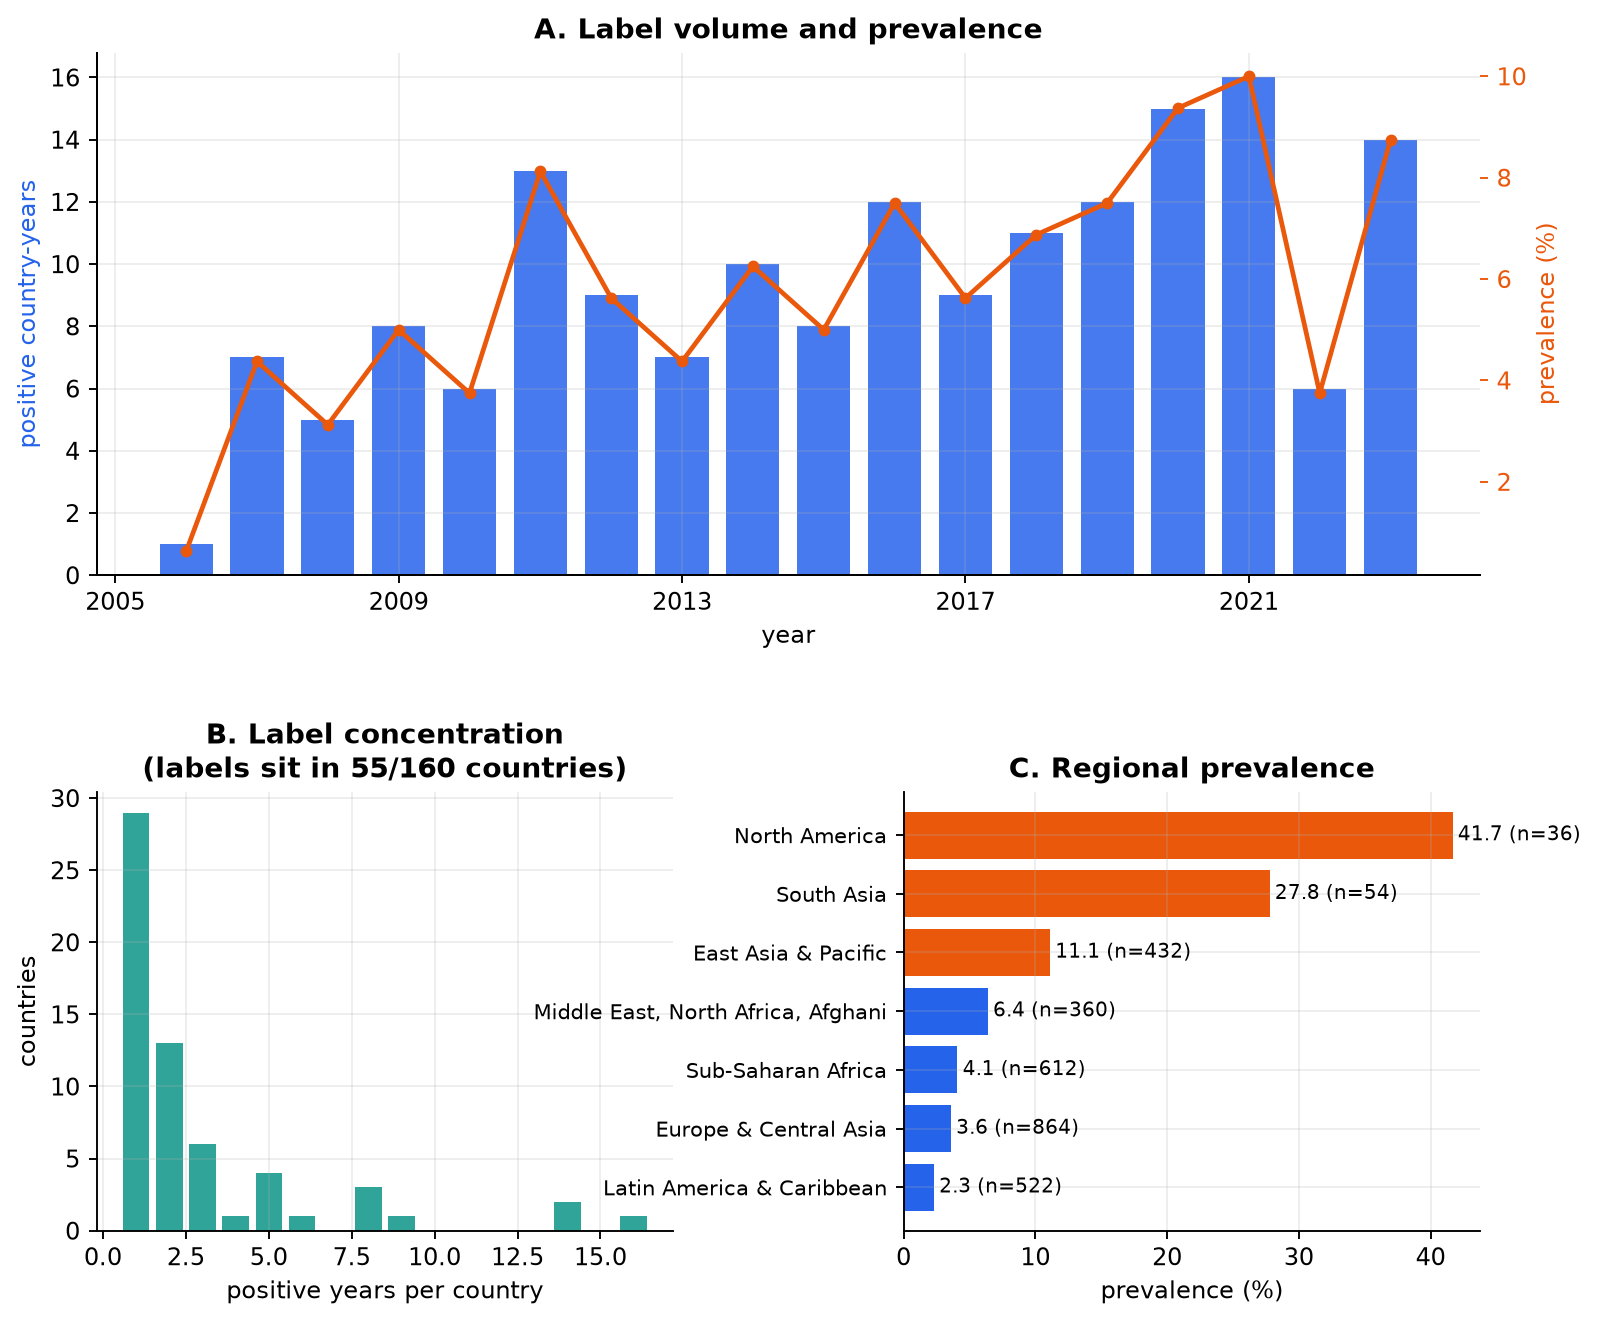
\includegraphics[width=\textwidth]{fig10_label_anatomy.png}
\caption{Label anatomy. Panel A gives annual positive counts against prevalence on the secondary
axis. Panel B gives the distribution of positive years per country. Panel C gives prevalence by
World Bank region.}
\label{fig:labels}
\end{figure}

Three properties shape the design. The imbalance, visible as the gap between the count and
prevalence axes in panel A, rules out accuracy as a metric. The persistence in panel B, with
30 of 55 positive countries recurring, justifies historical features. The
regional concentration in panel C is the first indication that the label tracks reporting capacity,
since those countries operate reference laboratories.

\subsection{Model Comparison}

Table~\ref{tab:level1} reports discrimination under all three schemes.

\begin{table}[htbp]
\centering
\caption{Discrimination at the country-year level. Brackets give 95 per cent bootstrap intervals
on the temporal holdout. Expected calibration error for the champion is 0.025 (Brier 0.0555).}
\label{tab:level1}
\small
\begin{tabular}{@{}lcccc@{}}
\toprule
\textbf{Model} & \textbf{PR-AUC (time)} & \textbf{95\% CI} & \textbf{ROC-AUC (time)} &
\textbf{PR-AUC (country)} \\
\midrule
Logistic regression & 0.461 & [0.34, 0.58] & 0.844 & 0.381 \\
Decision tree & 0.376 & [0.28, 0.48] & 0.871 & 0.243 \\
Random forest & 0.495 & [0.38, 0.62] & 0.874 & 0.322 \\
Extra trees & 0.494 & [0.38, 0.60] & 0.866 & 0.353 \\
XGBoost & 0.429 & [0.32, 0.54] & 0.846 & 0.268 \\
LightGBM & 0.471 & [0.36, 0.58] & 0.846 & 0.280 \\
\bottomrule
\end{tabular}
\end{table}

Two results need separating. On the forward temporal holdout the best discrimination comes from
Random forest at 0.495 against a base rate of 5.87\%, roughly a 8-fold lift. Under
leave-country-out validation the ranking inverts: Random forest falls to 0.322, while logistic
regression holds 0.381 and becomes the strongest model on the criterion that governs selection.
Its temporal score is 0.461, about a 8-fold lift.

Because deployment means an unseen country rather than an unseen year, the champion is
Logistic Regression. The inversion is the more informative result: with eight retained features the
relationships are close enough to additive that a regularised linear model transfers best, and the
flexible ensembles pay for their extra capacity in exactly the setting the project cares about. The
single decision tree is weakest on both schemes, which confirms that the signal is not concentrated
in one or two splits.

\section{Discussion}

All measured results above are for one task only: given features from year $t$, predict whether
glanders is documented in that country in year $t{+}1$. Logistic Regression reaches a
precision-recall AUC of 0.461 against a base rate of 5.87\% on the forward split, and holds 0.381
across unseen countries, with calibration error 0.025. The gap between those two figures is smaller
than the full-feature model showed, which is the practical gain from selecting features on
conditional evidence. The signal it learns is surveillance rather than biology: the leading features
are population, connectivity and reporting measures, the label concentrates in countries with
reference laboratories, and the best-scoring cells are India, the United States and Australia.

% =====================================================================
\chapter{Conclusion and Future Work}
\label{ch:concl}
% =====================================================================

\section{Conclusion}

This project set out to build a usable warning system for glanders: to establish whether
population-level risk could be predicted from public data, and how a prediction reaches the person who
owns the animals. Four sources new to the disease formed a country-year panel across 160
equine-holding countries, and six model families were trained under three validation schemes. Beside
the model, the platform is split into three components with fixed contracts: a risk engine, a RAG
question-answering layer and an alert service.

Prediction is possible, and the performance is moderate: Logistic Regression reaches a
precision-recall AUC of 0.461 against a base rate of 5.87\% on a forward split, about an 8-fold lift
with a calibration error of 0.025, and holds 0.381 across unseen countries. The skill is fragile
across geography, and the decline concentrates where early warning would help most.

What the model learns is less encouraging. Three analyses converge: the highest-ranked features are
population size and reporting capacity rather than biological drivers, the label concentrates in
countries operating reference laboratories, and the best-scoring cells have the strongest publishing
record. It predicts where glanders will be documented, not where it is.

\section{Limitations}
\label{sec:limitations}

The following limits apply to every headline number in this report.

\begin{enumerate}
  \item \textbf{The label is documentation, not incidence.} A positive means glanders was reported in
        the literature for that country-year; a negative may mean no disease or simply no report.
        Reporting effort is therefore the principal confounder: countries with reference laboratories
        and open-access publishing look riskier than countries with similar burden and weaker
        surveillance.
  \item \textbf{The extractor is unvalidated.} Occurrence events are reconstructed by an automated
        pipeline that has not been checked against a hand-annotated reference set, so extractor error
        is not separately quantified.
  \item \textbf{Few positives.} With 169 positive country-years the uncertainty on every metric is
        wide; bootstrap intervals are reported rather than hidden.
  \item \textbf{Country-year resolution only.} District-level modelling for India was not attempted,
        because public district covariates could not be assembled in time. Control is applied at a
        finer scale than the model predicts.
  \item \textbf{Not a clinical tool.} The model is population-level. It does not diagnose an
        individual animal and does not replace laboratory confirmation.
  \item \textbf{Geographic fragility.} Leave-country-out skill is weaker than temporal skill, and the
        drop is largest in regions where early warning would help most.
  \item \textbf{RAG and alerts are specified, not measured.} The RAG layer and alert service have
        interfaces, rules and evaluation protocols, but no deployed pilot scores. Monthly
        prediction, real SMS/WhatsApp delivery, and proof that recipients read or acted on a message
        remain future work (see also the alert-specific limits in Section~\ref{ch:alerts}).
\end{enumerate}

\section{Future Work}

\textbf{Reported activity.} The most important extension is to model surveillance capacity as a
quantity, as an offset on publication volume or a joint detection-and-occurrence model; otherwise gains in score reflect reporting, not disease.

\textbf{The label extractor.} The 263 extracted events have never been checked against a
hand-annotated set; annotating a stratified sample would give the extractor's own precision and
recall.

\textbf{Resolution and drift.} District-month resolution for India matches the scale at which
control is applied, but public district covariates would need assembling. The calibration here is one
point estimate, so production also needs drift monitoring and a retraining trigger.

\textbf{Measuring the RAG layer.} Its retrieval, guardrail and protocol targets are specified but
unmeasured. Running it against the corpus would give recall@5 and mean reciprocal rank for
retrieval, faithfulness and citation precision for grounding, and the out-of-scope refusal rate
against the false refusal rate in scope. Two further metrics matter in the field: answer usefulness,
rated by district officers on real questions rather than a hand-built set, and citation age, which
shows whether answers lean on guidance that has since been revised.

\textbf{Monthly alert operation.} Extend the ML pipeline to produce and validate monthly predictions, then integrate them through the alert service's period-aware prediction contract. Keep monthly and yearly alert states separate, and tune thresholds, hysteresis margins and cooldown windows for each frequency. Evaluate temporal leakage, reporting delays, seasonality, calibration and freshness before enabling monthly notifications.

\textbf{Production alert infrastructure.} Replace demonstration storage and single-process execution with durable PostgreSQL persistence, background workers and a reliable queue. Test event replay, concurrent evaluation, worker restarts and provider timeouts. Measure duplicate-alert prevention, queue recovery and end-to-end processing latency.

\textbf{Real notification channels.} Integrate approved SMS and WhatsApp providers for a consented pilot, while retaining the simulated or Telegram channel for development where appropriate. Complete provider onboarding and applicable message-template requirements. Measure provider acceptance, delivery receipts, latency, cost and failure reasons separately for each channel.

\textbf{Recipient acknowledgement and escalation.} Add an acknowledgement mechanism so the system can distinguish a message being sent from a warning being seen. Under a veterinary-approved policy, escalate unacknowledged HIGH alerts to the responsible veterinary officer or field worker. Evaluate acknowledgement time and follow-up completion in a supervised pilot.

\textbf{Low-connectivity reach.} Evaluate veterinary-officer and community field-worker relays, SMS and voice/IVR options for owners with limited smartphone or internet access. Measure whether warnings reach these recipients and whether the message is understood.

\textbf{Alert quality and field evaluation.} Evaluate the service separately for monthly and yearly operation using alert precision, false-alert rate, event coverage, missed-event rate, messages per recipient per month/year, delivery reliability per channel and time from alert to owner contact. Field studies should also assess whether recipients understand the warning and take appropriate veterinary or preventive action. These outcomes cannot be claimed until a real pilot with subscribers has been completed.

\textbf{Structured alert exchange.} If an external agency or partner requires interoperability, add an OASIS CAP export adapter for the structured alert record. Validate required fields and test exchange with a partner endpoint before claiming operational interoperability.

A WOAH WAHIS record set \cite{wahis} would validate the literature-derived label where the two
overlap, and a cost-sensitive threshold would match the operating point to programme priorities.

% ============================== REFERENCES ==============================
\newpage
\chapter*{Bibliography}
\addcontentsline{toc}{chapter}{Bibliography}
\renewcommand{\bibname}{}
\begin{multicols}{2}
\begin{thebibliography}{99}
\footnotesize
\setlength{\itemsep}{0.15em}
\setlength{\parskip}{0pt}
\bibitem{khan2013} Khan I, Wieler LH, Melzer F, et al. Glanders in animals: a review on epidemiology, clinical presentation, diagnosis and countermeasures. \emph{Transboundary and Emerging Diseases}. 2013. doi:10.1111/j.1865-1682.2012.01342.x
\bibitem{kanani2026} Kanani Y, Oryan A, Derakhshandeh A. Glanders: past, present and future of a neglected zoonosis as a threat in veterinary and human health. \emph{Veterinary Medicine and Science}. 2026. doi:10.1002/vms3.70950
\bibitem{purnama2026} Purnama MTE, Firdausy LW, Fikri F, et al. Seroprevalence and associated epidemiological drivers of glanders in horses: a systematic review and meta-analysis. \emph{Research in Veterinary Science}. 2026;106416. doi:10.1016/j.rvsc.2026.106416
\bibitem{mota2022} Mota RA, Pinheiro J\'unior JW. Current status of glanders in Brazil: recent advances and challenges. \emph{Brazilian Journal of Microbiology}. 2022. doi:10.1007/s42770-022-00814-1
\bibitem{singha2026} Singha H, Shanmugasundaram K, Jhandai P, et al. Surveillance of equine glanders in India (2019--2023): prevalence estimate, risk analysis and future strategy. \emph{Microbial Pathogenesis}. 2026;217:108597. doi:10.1016/j.micpath.2026.108597
\bibitem{singha2020} Singha H, Shanmugasundaram K, Tripathi BN, et al. Serological surveillance and clinical investigation of glanders among indigenous equines in India from 2015 to 2018. \emph{Transboundary and Emerging Diseases}. 2020. doi:10.1111/tbed.13475
\bibitem{malik2012} Malik P, Singha H, Khurana SK, et al. Emergence and re-emergence of glanders in India: a description of outbreaks from 2006 to 2011. \emph{Veterinaria Italiana}. 2012. PMID:22718333
\bibitem{fonseca2019} Fonseca-Rodr\'iguez O, Pinheiro J\'unior JW, Mota RA. Spatiotemporal analysis of glanders in Brazil. \emph{Journal of Equine Veterinary Science}. 2019. doi:10.1016/j.jevs.2019.03.216
\bibitem{moawad2019} Moawad AA, Silge A, Bocklitz T, Fischer K, R\"osch P, Roesler U, Elschner MC, Popp J, Neubauer H. A machine learning-based Raman spectroscopic assay for the identification of \emph{Burkholderia mallei} and related species. \emph{Molecules}. 2019;24(24):4516. doi:10.3390/molecules24244516
\bibitem{stoeckel2015} St\"ockel S, Meisel S, Elschner M, Melzer F, R\"osch P, Popp J. Raman spectroscopic detection and identification of \emph{Burkholderia mallei} and \emph{Burkholderia pseudomallei}. \emph{Analytical and Bioanalytical Chemistry}. 2015;407(3):833--843. doi:10.1007/s00216-014-7906-5
\bibitem{collier2012} Collier N. Uncovering text mining: a survey of current work on web-based epidemic intelligence. \emph{Global Public Health}. 2012. doi:10.1080/17441692.2012.699975
\bibitem{lejeune2015} Lejeune G, Brixtel R, Doucet A, et al. Multilingual event extraction for epidemic detection. \emph{Artificial Intelligence in Medicine}. 2015. doi:10.1016/j.artmed.2015.06.005
\bibitem{chen2016} Chen T, Guestrin C. XGBoost: a scalable tree boosting system. In: \emph{Proceedings of the 22nd ACM SIGKDD International Conference on Knowledge Discovery and Data Mining}. 2016:785--794. doi:10.1145/2939672.2939785
\bibitem{ke2017} Ke G, Meng Q, Finley T, et al. LightGBM: a highly efficient gradient boosting decision tree. In: \emph{Advances in Neural Information Processing Systems 30 (NIPS)}. 2017:3146--3154.
\bibitem{breiman2001} Breiman L. Random forests. \emph{Machine Learning}. 2001. doi:10.1023/A:1010933404324
\bibitem{lundberg2017} Lundberg SM, Lee SI. A unified approach to interpreting model predictions. In: \emph{Advances in Neural Information Processing Systems 30 (NIPS)}. 2017:4765--4774. arXiv:1705.07874
\bibitem{saito2015} Saito T, Rehmsmeier M. The precision-recall plot is more informative than the ROC plot when evaluating binary classifiers on imbalanced datasets. \emph{PLOS ONE}. 2015;10(3):e0118432. doi:10.1371/journal.pone.0118432
\bibitem{davis2006} Davis J, Goadrich M. The relationship between precision-recall and ROC curves. In: \emph{Proceedings of the 23rd International Conference on Machine Learning}. 2006:233--240. doi:10.1145/1143844.1143874
\bibitem{roberts2017} Roberts DR, Bahn V, Ciuti S, et al. Cross-validation strategies for data with temporal, spatial, hierarchical, or phylogenetic structure. \emph{Ecography}. 2017. doi:10.1111/ecog.02881
\bibitem{niculescu2005} Niculescu-Mizil A, Caruana R. Predicting good probabilities with supervised learning. In: \emph{Proceedings of the 22nd International Conference on Machine Learning}. 2005:625--632. doi:10.1145/1102351.1102430
\bibitem{huang2020} Huang Y, Li W, Macheret F, et al. A tutorial on calibration measurements and calibration models for clinical prediction models. \emph{Journal of the American Medical Informatics Association}. 2020;27(4):621--633. doi:10.1093/jamia/ocz228
\bibitem{lewis2020} Lewis P, Perez E, Piktus A, et al. Retrieval-augmented generation for knowledge-intensive NLP tasks. In: \emph{Advances in Neural Information Processing Systems 33 (NeurIPS)}. 2020:9459--9474. arXiv:2005.11401
\bibitem{reimers2019} Reimers N, Gurevych I. Sentence-BERT: sentence embeddings using Siamese BERT-networks. In: \emph{Proceedings of the 2019 Conference on Empirical Methods in Natural Language Processing (EMNLP-IJCNLP)}. 2019:3982--3992. doi:10.18653/v1/D19-1410
\bibitem{malkov2020} Malkov YA, Yashunin DA. Efficient and robust approximate nearest neighbor search using hierarchical navigable small world graphs. \emph{IEEE Transactions on Pattern Analysis and Machine Intelligence}. 2020;42(4):824--836. doi:10.1109/TPAMI.2018.2889473
\bibitem{robertson2009} Robertson S, Zaragoza H. The probabilistic relevance framework: BM25 and beyond. \emph{Foundations and Trends in Information Retrieval}. 2009;3(4):333--389. doi:10.1561/1500000019
\bibitem{cormack2009} Cormack GV, Clarke CLA, Buettcher S. Reciprocal rank fusion outperforms Condorcet and individual rank learning methods. In: \emph{Proceedings of the 32nd International ACM SIGIR Conference}. 2009:758--759. doi:10.1145/1571941.1572114
\bibitem{pedregosa2011} Pedregosa F, Varoquaux G, Gramfort A, et al. Scikit-learn: machine learning in Python. \emph{Journal of Machine Learning Research}. 2011;12:2825--2830.
\bibitem{wahis} WOAH. World Animal Health Information System (WAHIS). \url{https://wahis.woah.org}
\bibitem{dahd2025} Department of Animal Husbandry and Dairying, Government of India. \emph{National Action Plan for Control and Eradication of Glanders in India} (Revised 2025). New Delhi: DAHD; 2025.
\bibitem{faostat} FAO. FAOSTAT: crops and livestock products. \url{https://www.fao.org/faostat}
\bibitem{power} NASA Langley Research Center. POWER agroclimatology API. \url{https://power.larc.nasa.gov}
\bibitem{wdi} World Bank. World Development Indicators. \url{https://databank.worldbank.org}
\bibitem{europepmc} Europe PMC literature search API. \url{https://europepmc.org}
\bibitem{nadres} ICAR-National Institute of Veterinary Epidemiology and Disease Informatics. National Animal Disease Referral Expert System (NADRES v2): livestock disease forecasting. \url{https://nivedi.res.in/Nadres_v2/}
\end{thebibliography}
\end{multicols}


\end{document}
